\clearpage
\begin{savequote}[8cm]
\textlatin{Neque porro quisquam est qui dolorem ipsum quia dolor sit amet, consectetur, adipisci velit...}

There is no one who loves pain itself, who seeks after it and wants to have it, simply because it is pain...
  \qauthor{--- Cicero's \textit{de Finibus Bonorum et Malorum}}
\end{savequote}

\chapter{\label{ch:5-massfit}Mass fit} 

\minitoc

\section{Mass parameterisation of the favoured mode}
\label{sec:massfit}

The fit to data is performed on the invariant mass of B candidates. Firstly a fit model was developed and applied to the favoured mode, namely \decay{\Bm}{\D(\Km\pip)\Kstarm}.

\subsection{Signal shape}
\label{sec:massfit:signal}

The signal shape is constructed using the sum of two Crystal Ball (CB) functions~\cite{Skwarnicki:1986xj}, where the tail parameters, $\alpha$ and $n$, are fixed from MC and both CBs share the same mean and tail parameters. This Double Crystal Ball shape is defined in Equation \ref{DCBshape}. The width fraction between the CBs, $f_{\sigma}$, is fixed from MC, but the mean and width, $\mu$ and $\sigma$, are left floating. 

\begin{equation}
\mathrm{DCB}(m; \mu,\sigma,\alpha,n,f_{cb}) = f_{cb} \cdot \mathrm{CB}(m; \mu,\sigma,\alpha,n) + (1-f_{cb}) \cdot \mathrm{CB}(m;\mu,f_{\sigma}\sigma,\alpha,n),
\label{DCBshape}
\end{equation}
where
\begin{equation*}
  \mathrm{CB}(m; \mu,\sigma,\alpha,n)=
\begin{cases}
    e^{-((m-\mu)/ \sigma)^2/2},                                   & \text{if } \frac{m-\mu}{\sigma} \geq - \alpha, \\
   \left ( \frac{n}{|\alpha|} \right ) ^n e^{-|\alpha|^2/2} \left ( \frac{n}{|\alpha|} - |\alpha| - \left ( \frac{m-\mu}{\sigma} \right ) \right ) ^{-n} ,    & \text{otherwise.}
\end{cases}
\end{equation*}


The fits to signal MC are shown in Figure \ref{signalfits} and the shape parameters obtained from these fits are detailed in Table \ref{signalparameters}. 
%The fitted mean value in data and MC was found to be slightly different, the values of the differences are shown in Table \ref{mcshifts}.

\begin{figure}[h]
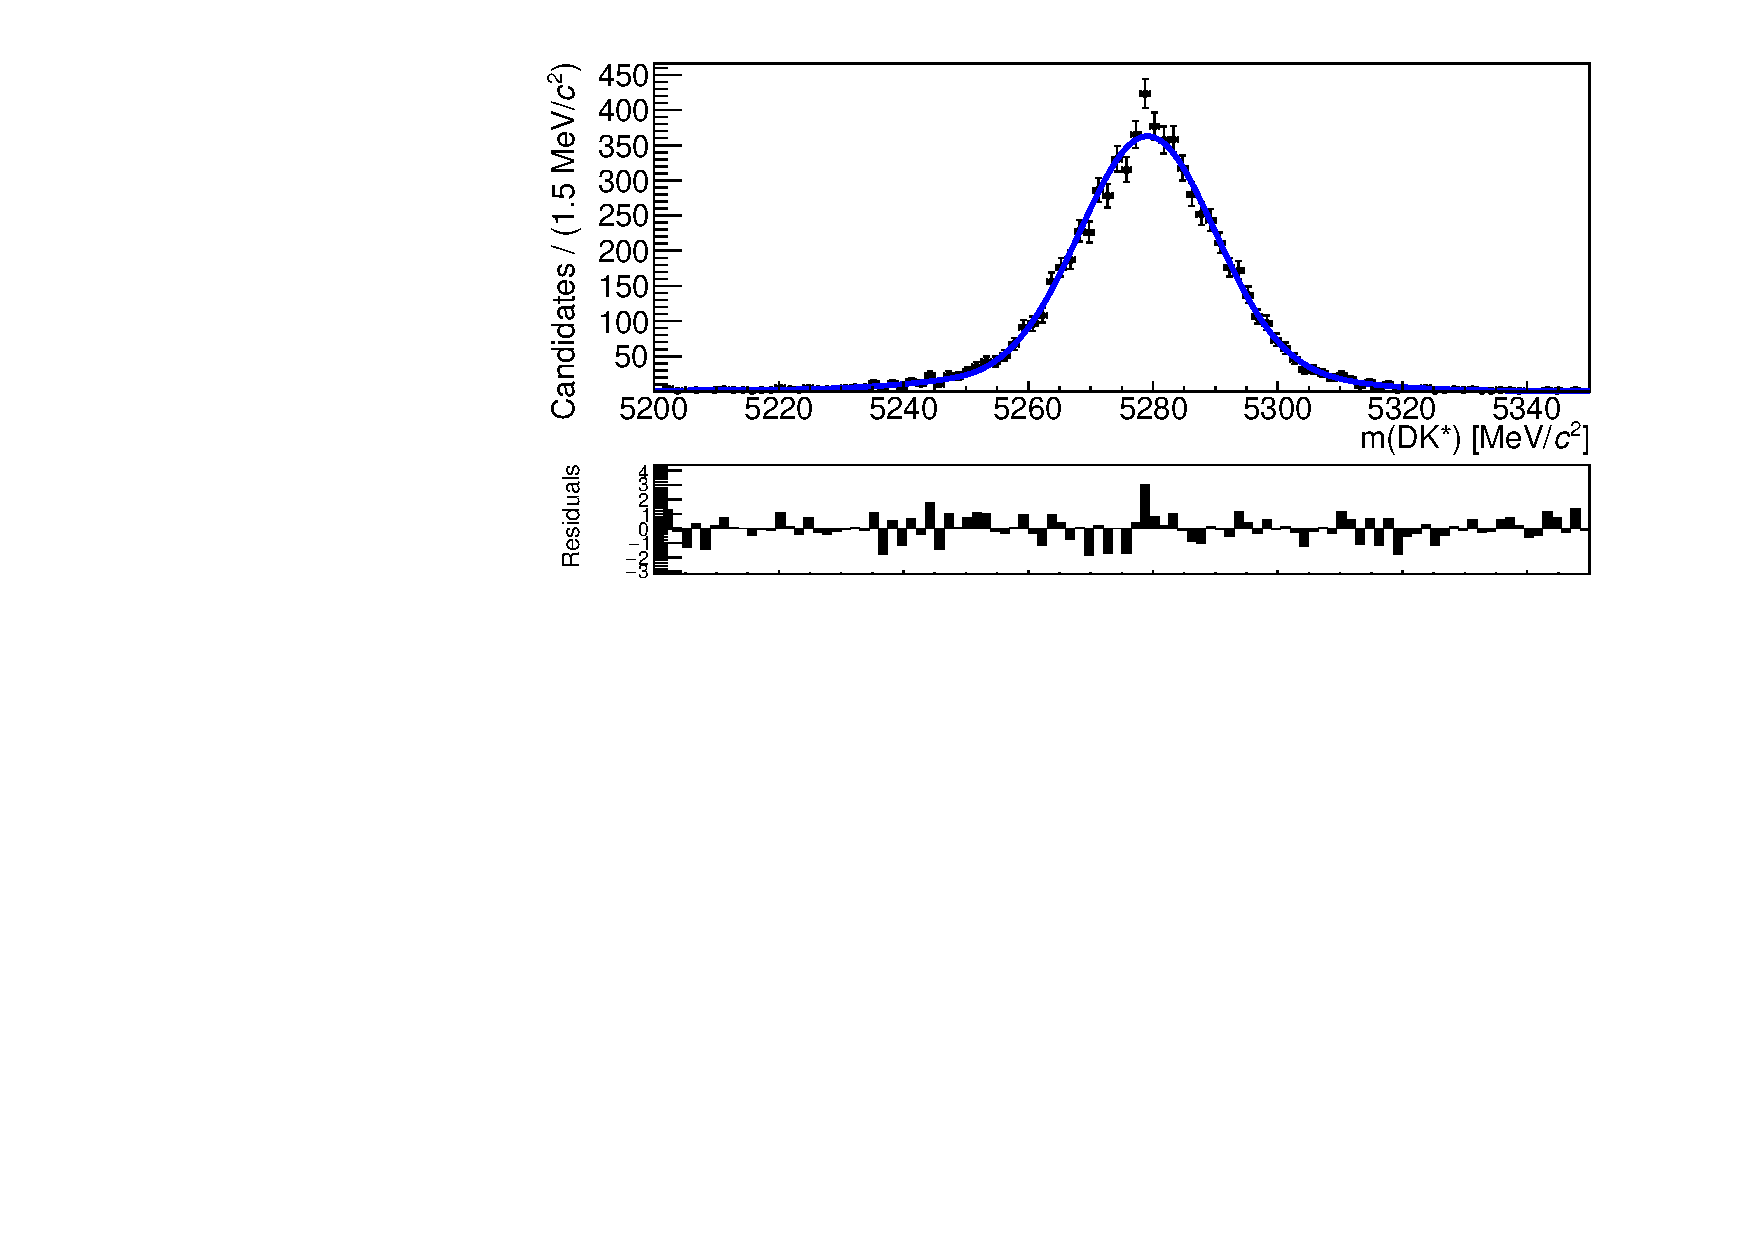
\includegraphics[width=0.5\linewidth]{figures/fitComponents/signalShape_LL_KPi.pdf}
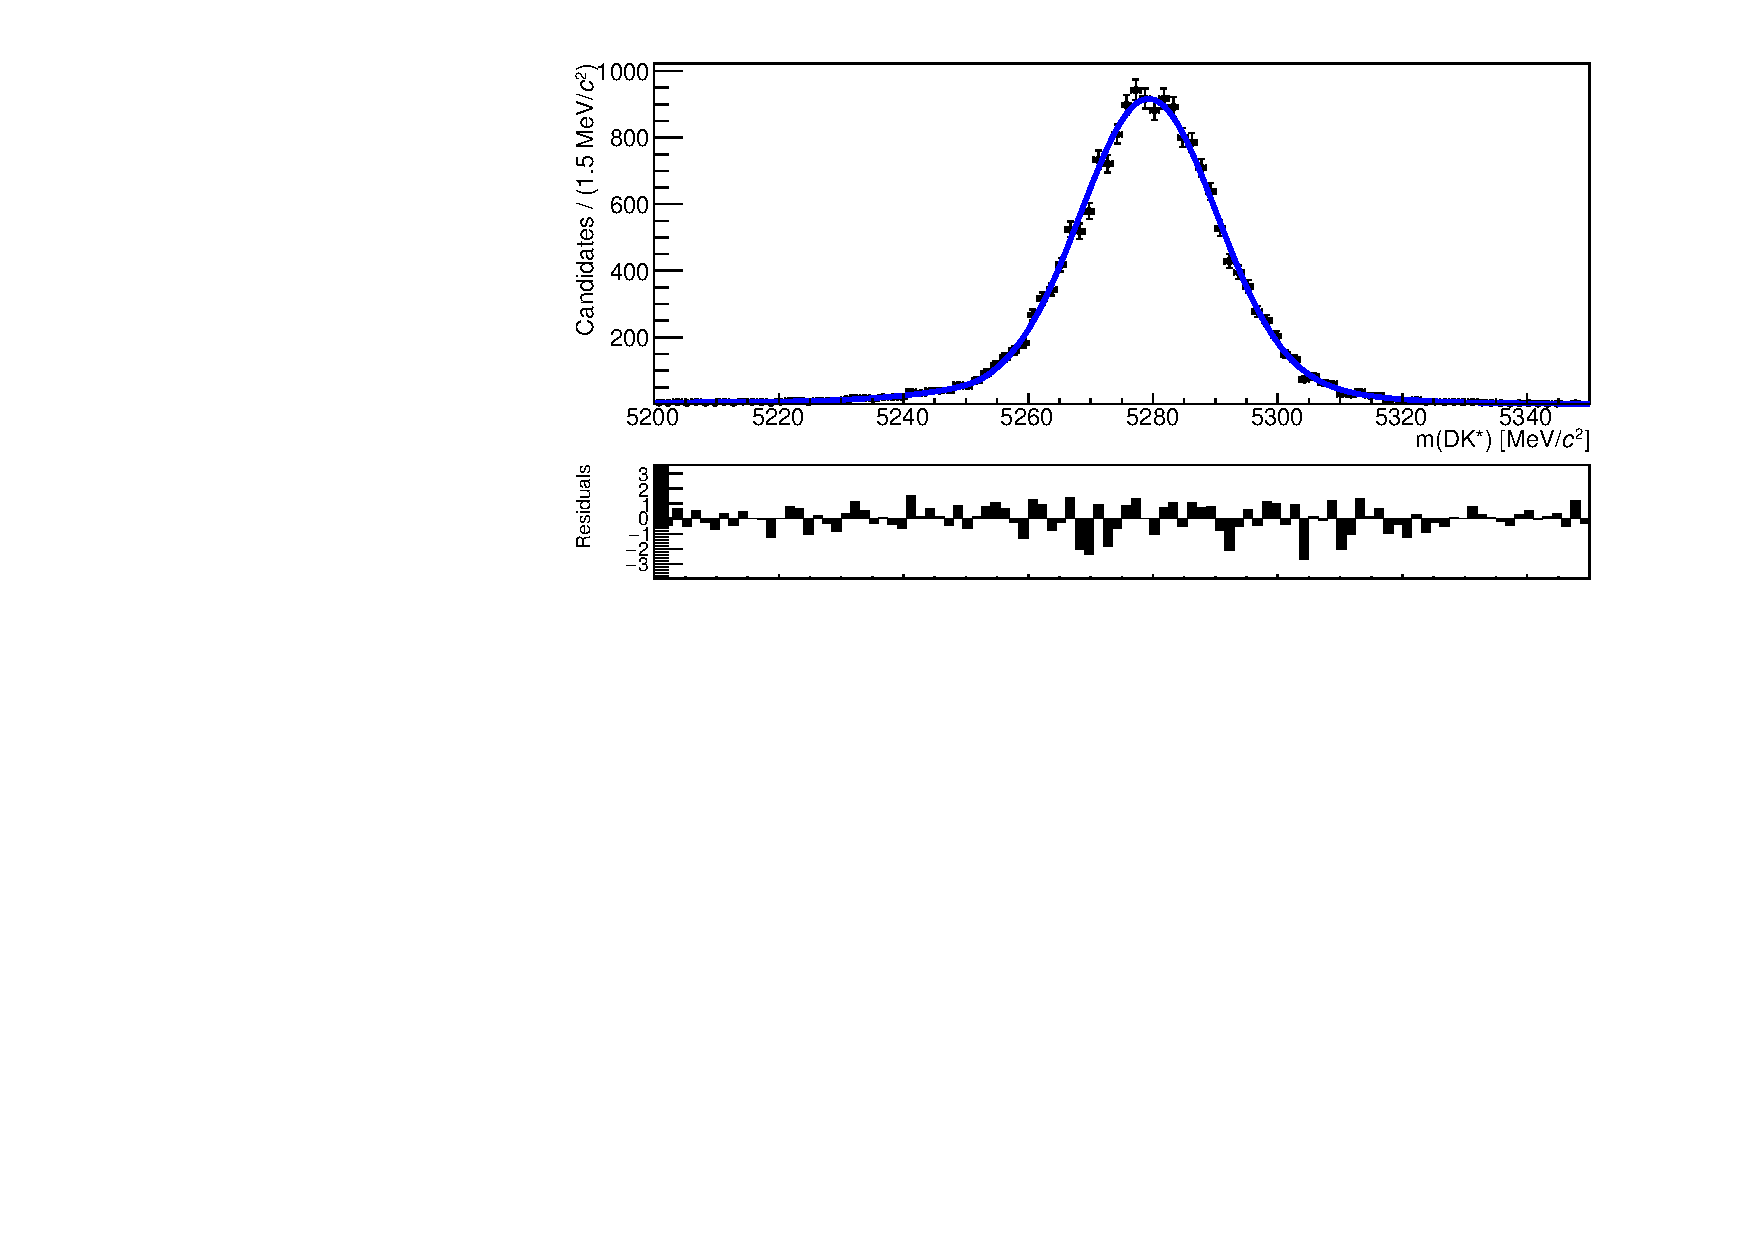
\includegraphics[width=0.5\linewidth]{figures/fitComponents/signalShape_DD_KPi.pdf}
\put(-400,70) {(a)}
\put(-180,70) {(b)}
\hfill
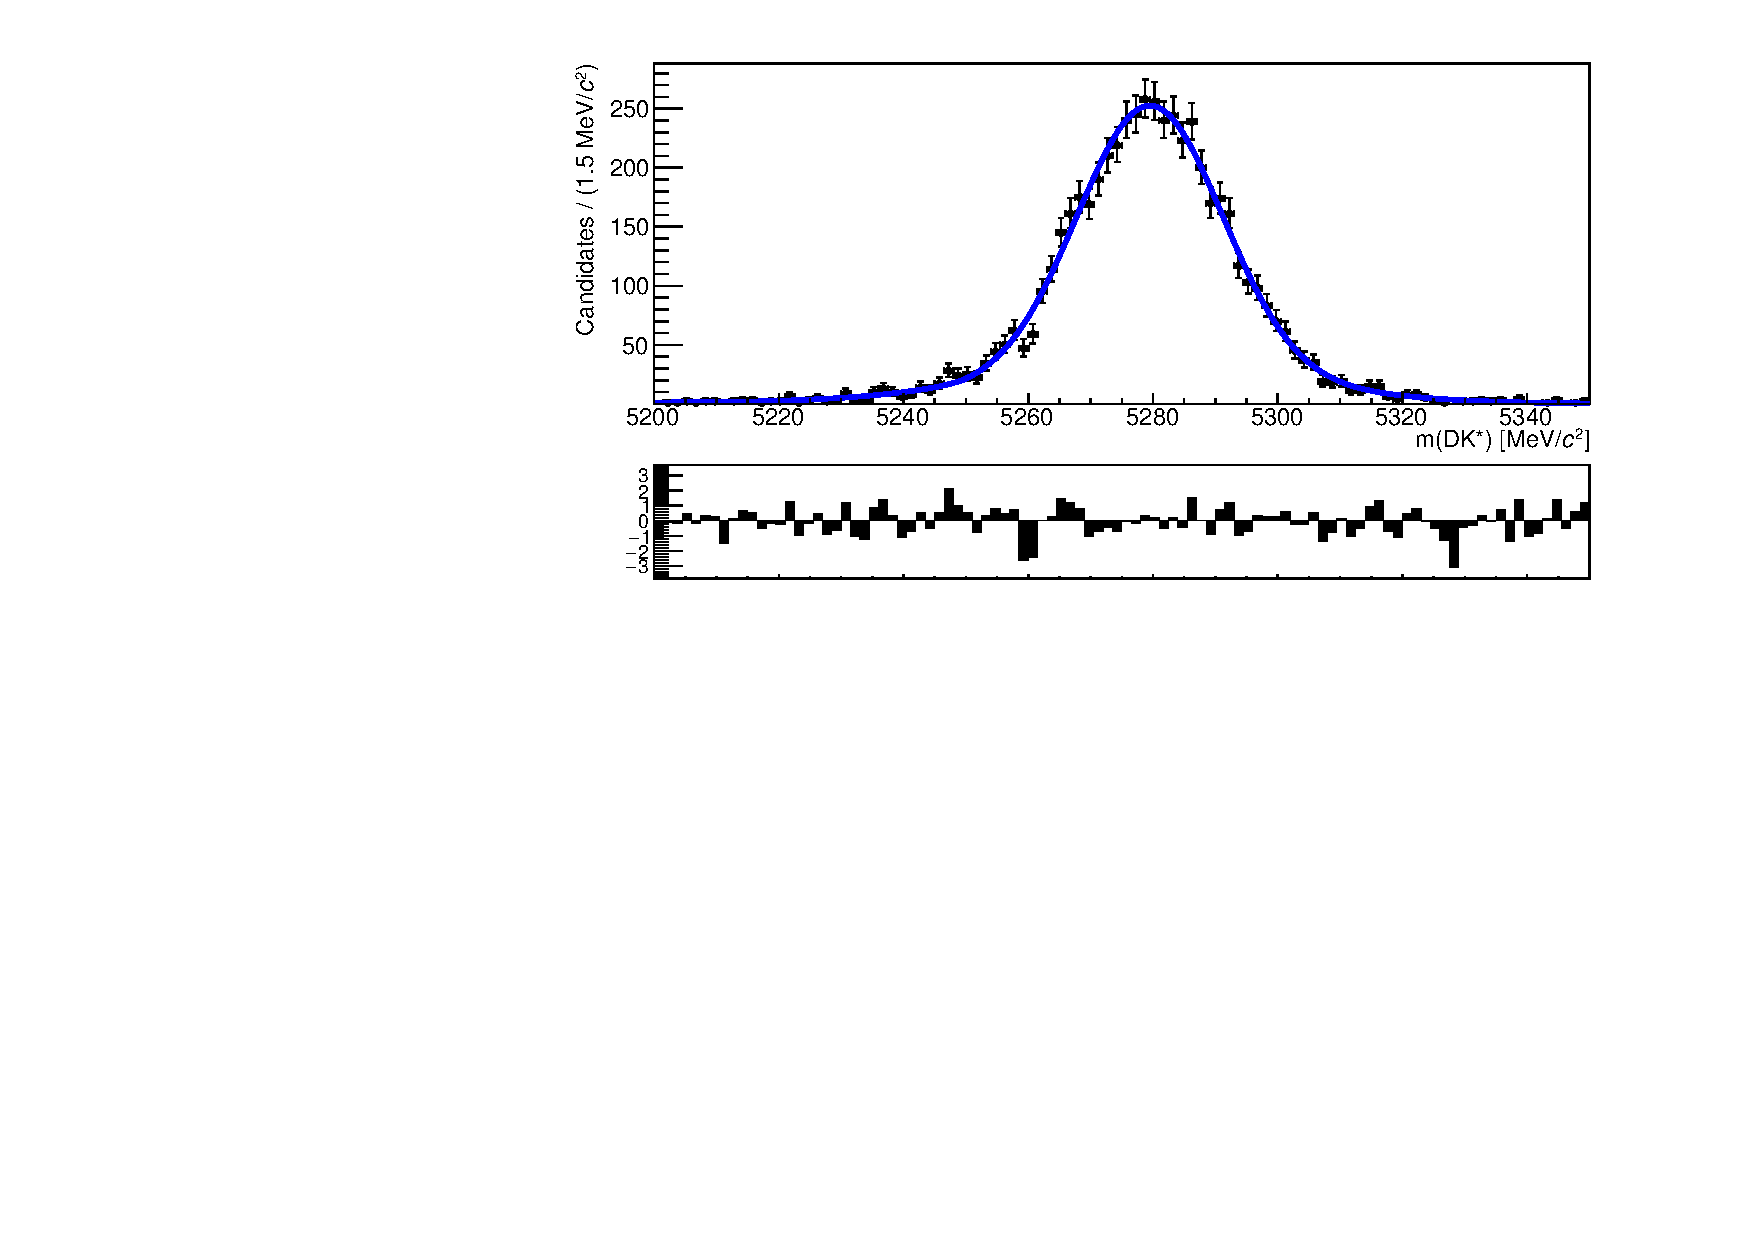
\includegraphics[width=0.5\linewidth]{figures/fitComponents/signalShape_LL_KPiPiPi.pdf}
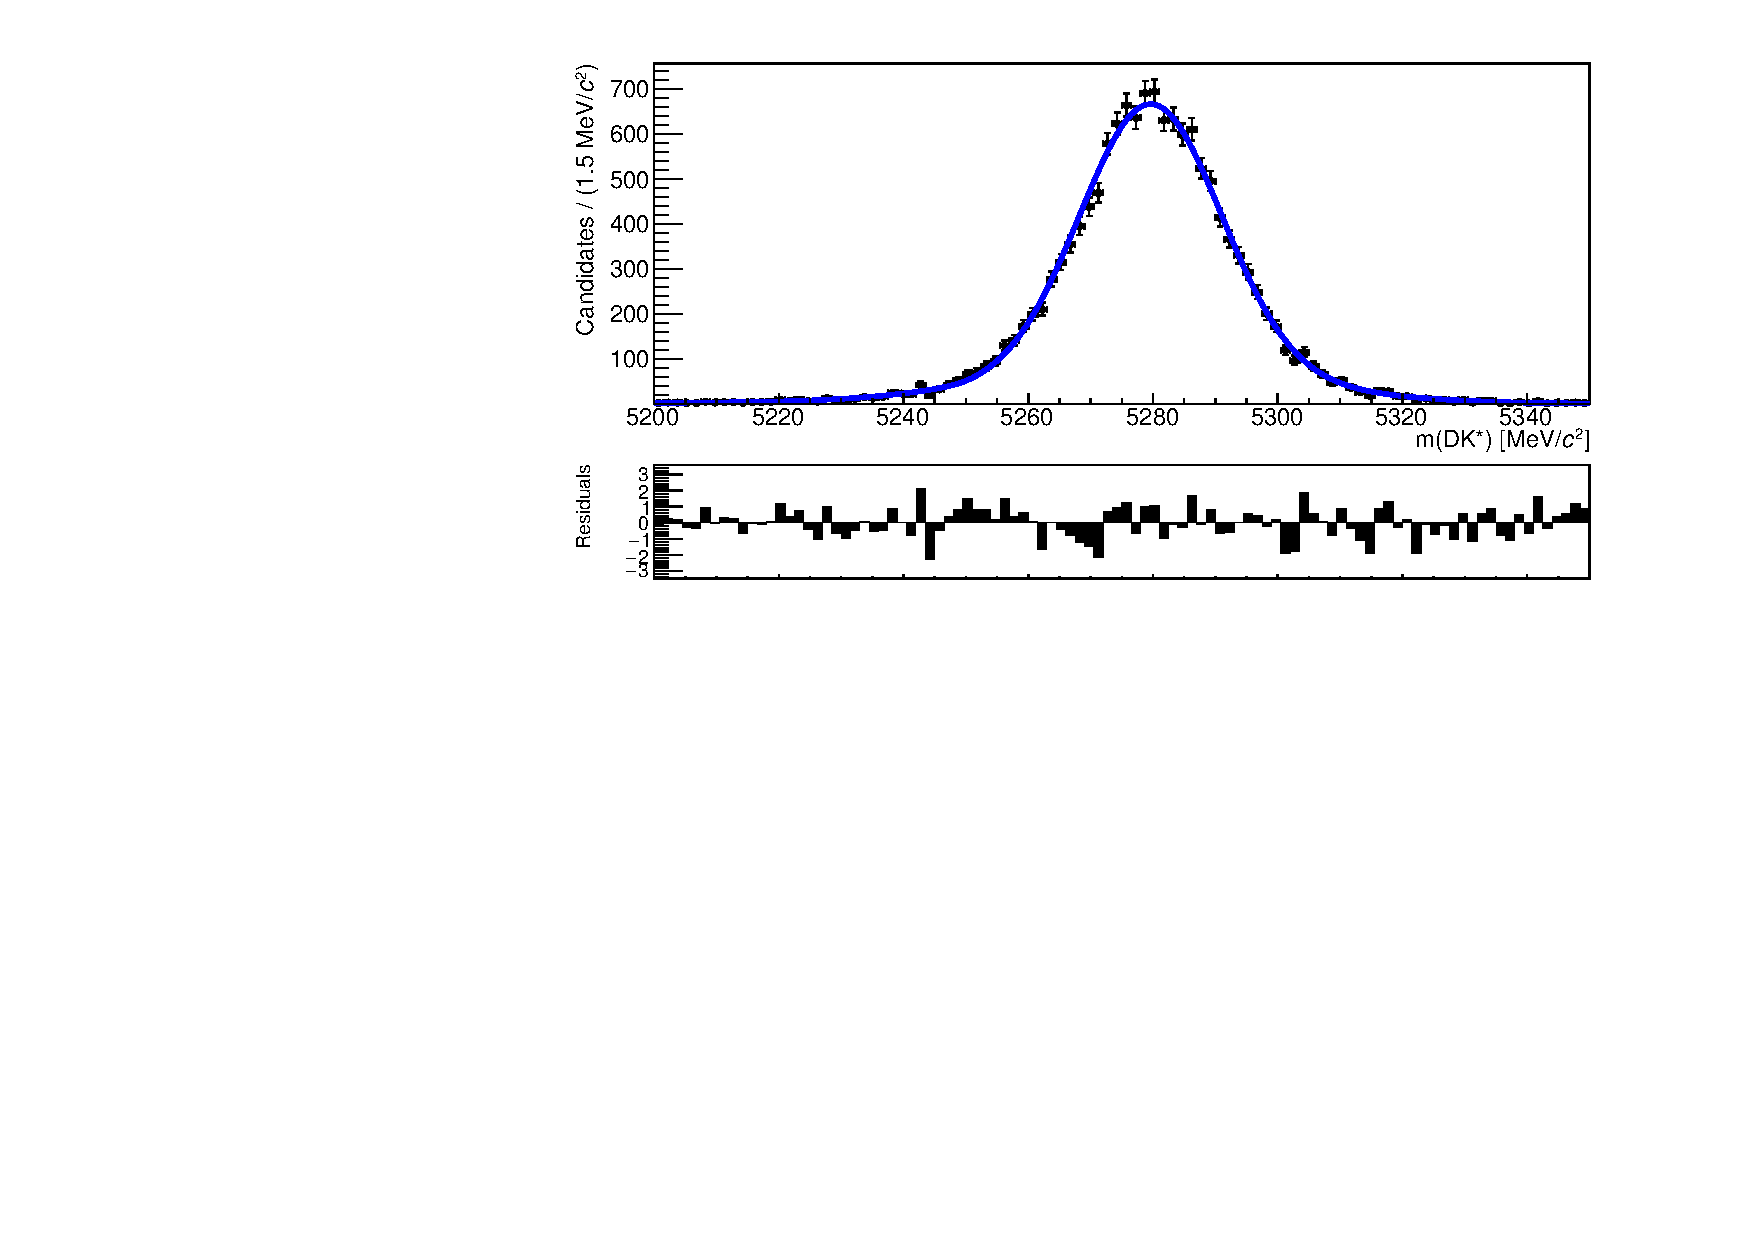
\includegraphics[width=0.5\linewidth]{figures/fitComponents/signalShape_DD_KPiPiPi.pdf}
\put(-400,70) {(c)}
\put(-180,70) {(d)}
\caption{Fits to signal MC for (a) $K\pi$ LL, (b) $K\pi$ DD, (c) $K\pi\pi\pi$ LL, and (d) $K\pi\pi\pi$ DD}
\label{signalfits}
\end{figure}

\begin{table}[h]
\centering
\begin{tabular}{c|cc|cc}
\hline
& \multicolumn{2}{c}{$K\pi$} & \multicolumn{2}{c}{$K\pi\pi\pi$} \\
& LL & DD & LL & DD\\
\hline
$\mu$ & $5279.12 \pm 0.15$ & $5279.30 \pm 0.09$ & $5279.62 \pm 0.12$ & $5279.50 \pm 0.19$ \\
$\sigma$ & $10.7 \pm 0.3$ & $10.8 \pm 0.2$ & $11.2 \pm 0.2$ & $11.6 \pm 0.3$ \\
$f_{\sigma}$ & $2.04 \pm 0.10$ & $1.97 \pm 0.06$ & $2.08 \pm 0.07$ & $2.10 \pm 0.11$ \\
$\alpha$ & $2.53 \pm 0.07$ & $2.46 \pm 0.04$ & $2.60 \pm 0.07$ & $2.50 \pm 0.10$ \\
$n$ & 1.0 (fixed) & 1.0 (fixed) & 1.0 (fixed) & 1.0 (fixed) \\
$f_{cb}$ & $0.82 \pm 0.03$ & $0.84 \pm 0.02$ & $0.80 \pm 0.03$ & $0.81 \pm 0.04	$ \\
\hline
\end{tabular}
\caption{Signal shape parameters obtained by a fit to Run 1 and Run 2 signal MC combined for both $K\pi$ and $K\pi\pi\pi$. Parameter names are defined in Equation \ref{DCBshape}. All parameters except for the mean and width are fixed to these values in the mass fit}
\label{signalparameters}
\end{table}

%\begin{table}
%\centering
%\begin{tabular}{ccc}
%\hline
%& Run 1 & 2015 \\
%\hline
%LL & +1.5 & +1.2 \\
%DD & +0.4 & 0.0 \\
%\hline
%\end{tabular}
%\caption{Difference (in MeV) in the fitted value of the mean between data and MC (data - MC)}
%\label{mcshifts}
%\end{table}


\subsection{Combinatorial background}
\label{sec:massfit:combinatorial}

The combinatoric background is modelled using an exponential function with a freely floating slope parameter and yield. The slope parameter is allowed to float independently in the LL and DD categories and between 2 and 4 body D final states. Each D final state can have a different combinatoric rate.


%%%%%%%%%%%%%%%%%%%%%%
\subsection{Partially reconstructed backgrounds}
\label{sec:massfit:partreco}

The partially reconstructed decays are of the form \decay{\B}{\Dstar\Kstar}, where the \Dstar decays to a \D meson and a pion or photon that is missed in reconstruction. These backgrounds are observed at a low reconstructed invariant mass due to the single particle missed from the invariant mass sum. Three partially reconstructed decays contribute in the invariant mass fit:

\begin{itemize}
\item{\decay{\Bm}{(\decay{\Dstarz}{\Dz[\piz]})\Kstarm}}
\item{\decay{\Bm}{(\decay{\Dstarz}{\Dz[\gamma]})\Kstarm}}
\item{\decay{\Bd}{(\decay{\Dstarp}{\Dz[\pip]})\Kstarm}}
\end{itemize}

where the particle in square brackets corresponds to the missing daughter. All of the decay modes listed are modelled using three analytic PDFs; RooHORNSdini, RooHILLdini and RooLITTLEHORNSdini. These PDFs are physically motivated, exploiting the decay kinematics of partially reconstructed decays. These PDFs are described in more detail in the \decay{\Bz}{\D	\Kstarz} GGSZ analysis note~\cite{B02DKst0_GGSZ}.

\decay{\Bm}{\Dstarp\Kstarm} is a Scalar $\to$ Vector Vector decay, therefore there are three different helicity amplitudes to consider due to the conservation of angular momentum. Each of these helicity amplitudes produces a \Dstar particle in a different helicity state. The three helicity amplitudes are referred to as 001, 010 and 100, which correspond to helicity states shown in Table \ref{helicityamplitudes}. 

\begin{table}[h]
\centering
\begin{tabular}{c|ccc}
\hline
& B (J=0) & \Dstar (J=1) & \Kstar (J=1) \\
\hline
001 & 0 & -1 & +1 \\
010 & 0 & 0 & 0 \\
100 & 0 & +1 & -1 \\
\end{tabular}
\caption{Possible helicity amplitudes of the \decay{\B}{\Dstar\Kstar} decay. The numbers in the table correspond $J_z$ values}
\label{helicityamplitudes}
\end{table}

The \B mass distribution of these decays depends on the helicity amplitude of the decay and the spin of the missing particle. For each decay amplitude the spin of the helicity angle of the missing particle has a one-to-one correspondance with the missing momentum and therefore to the reconstructed \B mass. 

The \B mass distribution will not only depend on the physics of the decay but also on selection and reconstruction effects. Reconstruction and selection favours decays with higher reconstructed \B mass, the selection efficiency can be modelled by linear function with a slope parameter. In order to model detector effects, the shapes are convolved with a resolution function, described by a double Gaussian.

For each partially reconstructed background, the generated MC for 001 and 100 helicity amplitudes is physically indistiguishable in B mass and so these are combined to form a 101 helicity ampltiude. For each shape 1M events were generated and stripping and selection was applied, except for the PID selection. The shapes are taken from MC are fitted separately using the RooHORNSdini, RooHILLdini and RooLITTLEHORNSdini, the fits are shown in Figures \ref{partrecofitsLL} and \ref{partrecofitsDD}. All the parameters for these shapes are fixed in the mass fit from fits to MC.

\begin{figure}[h]
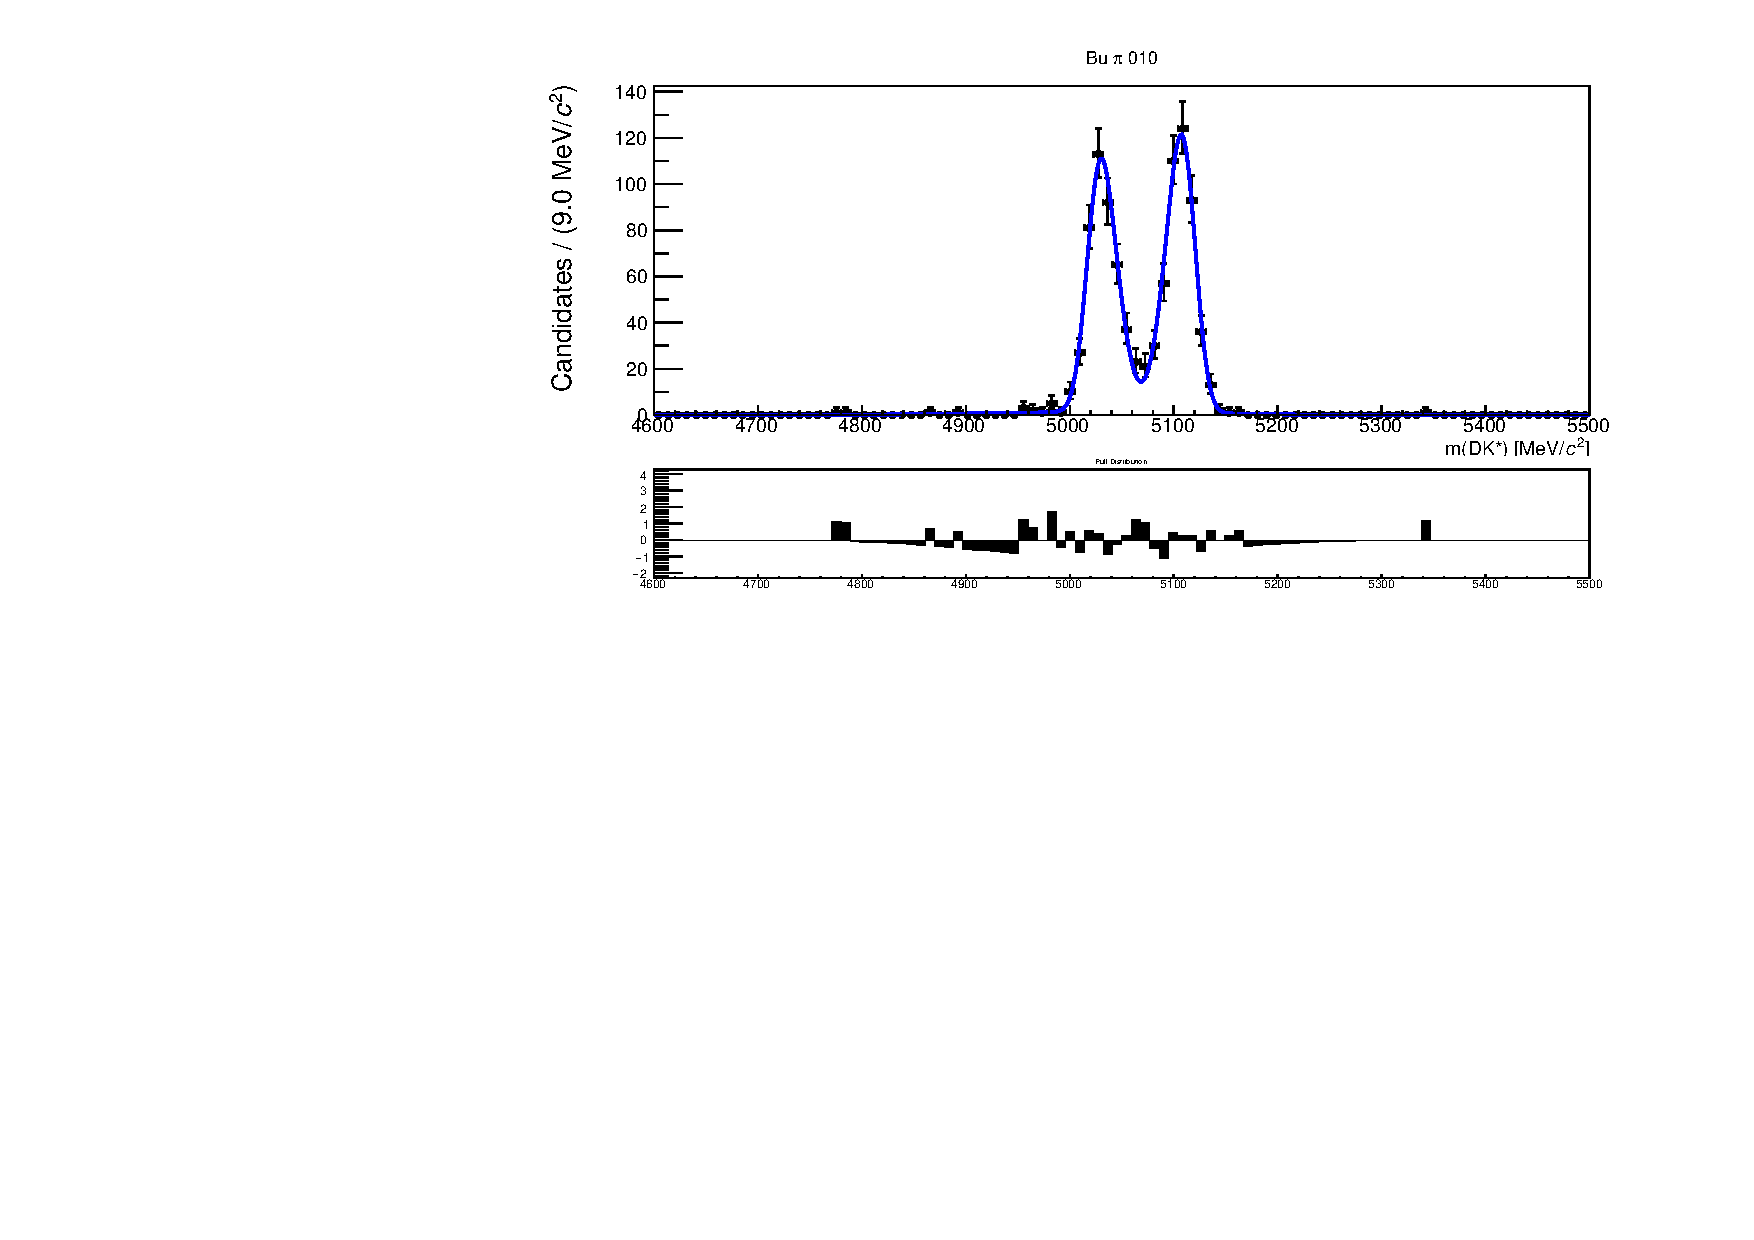
\includegraphics[width=0.5\linewidth]{figures/fitComponents/Bupi010_LL.pdf}
\put(-180,80) {(a)}
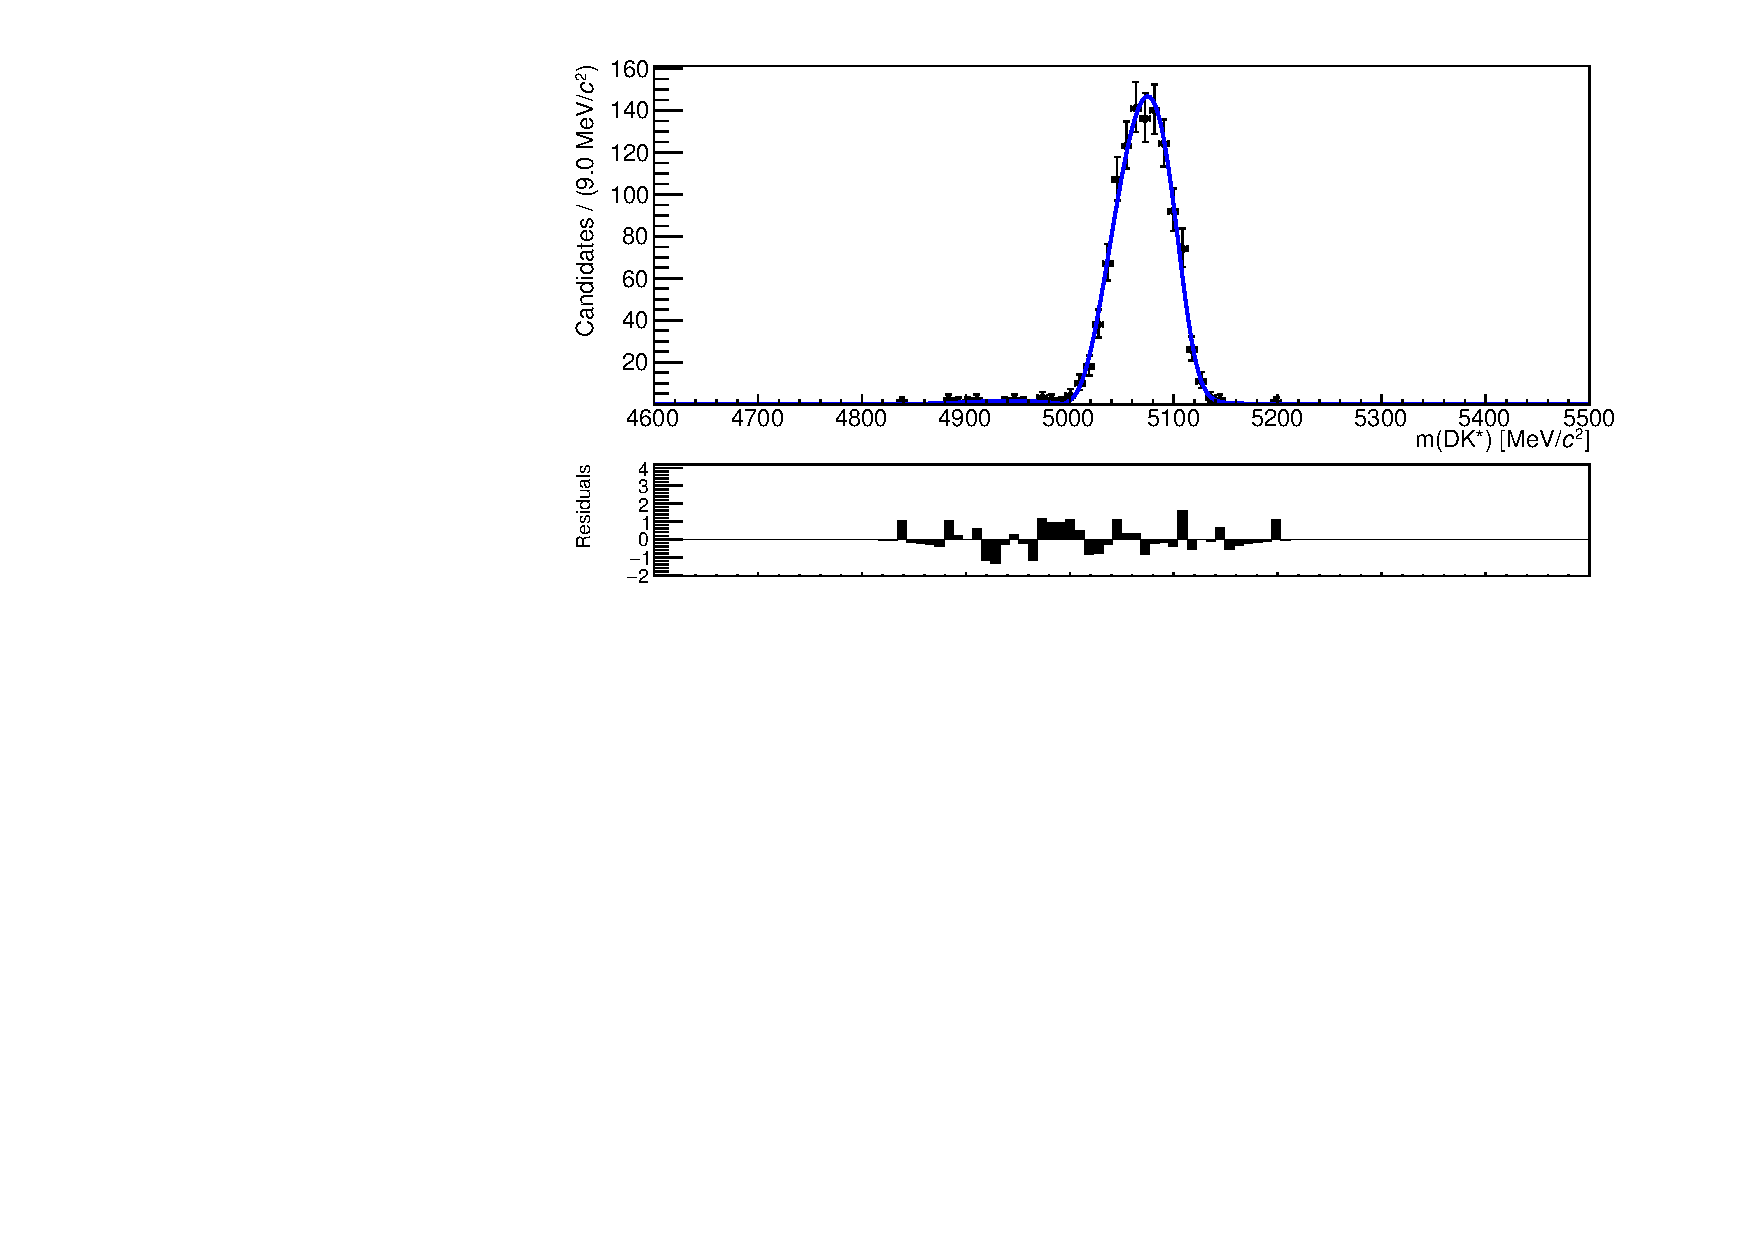
\includegraphics[width=0.5\linewidth]{figures/fitComponents/Bupi101_LL.pdf}
\put(-180,80) {(b)}
\hfill
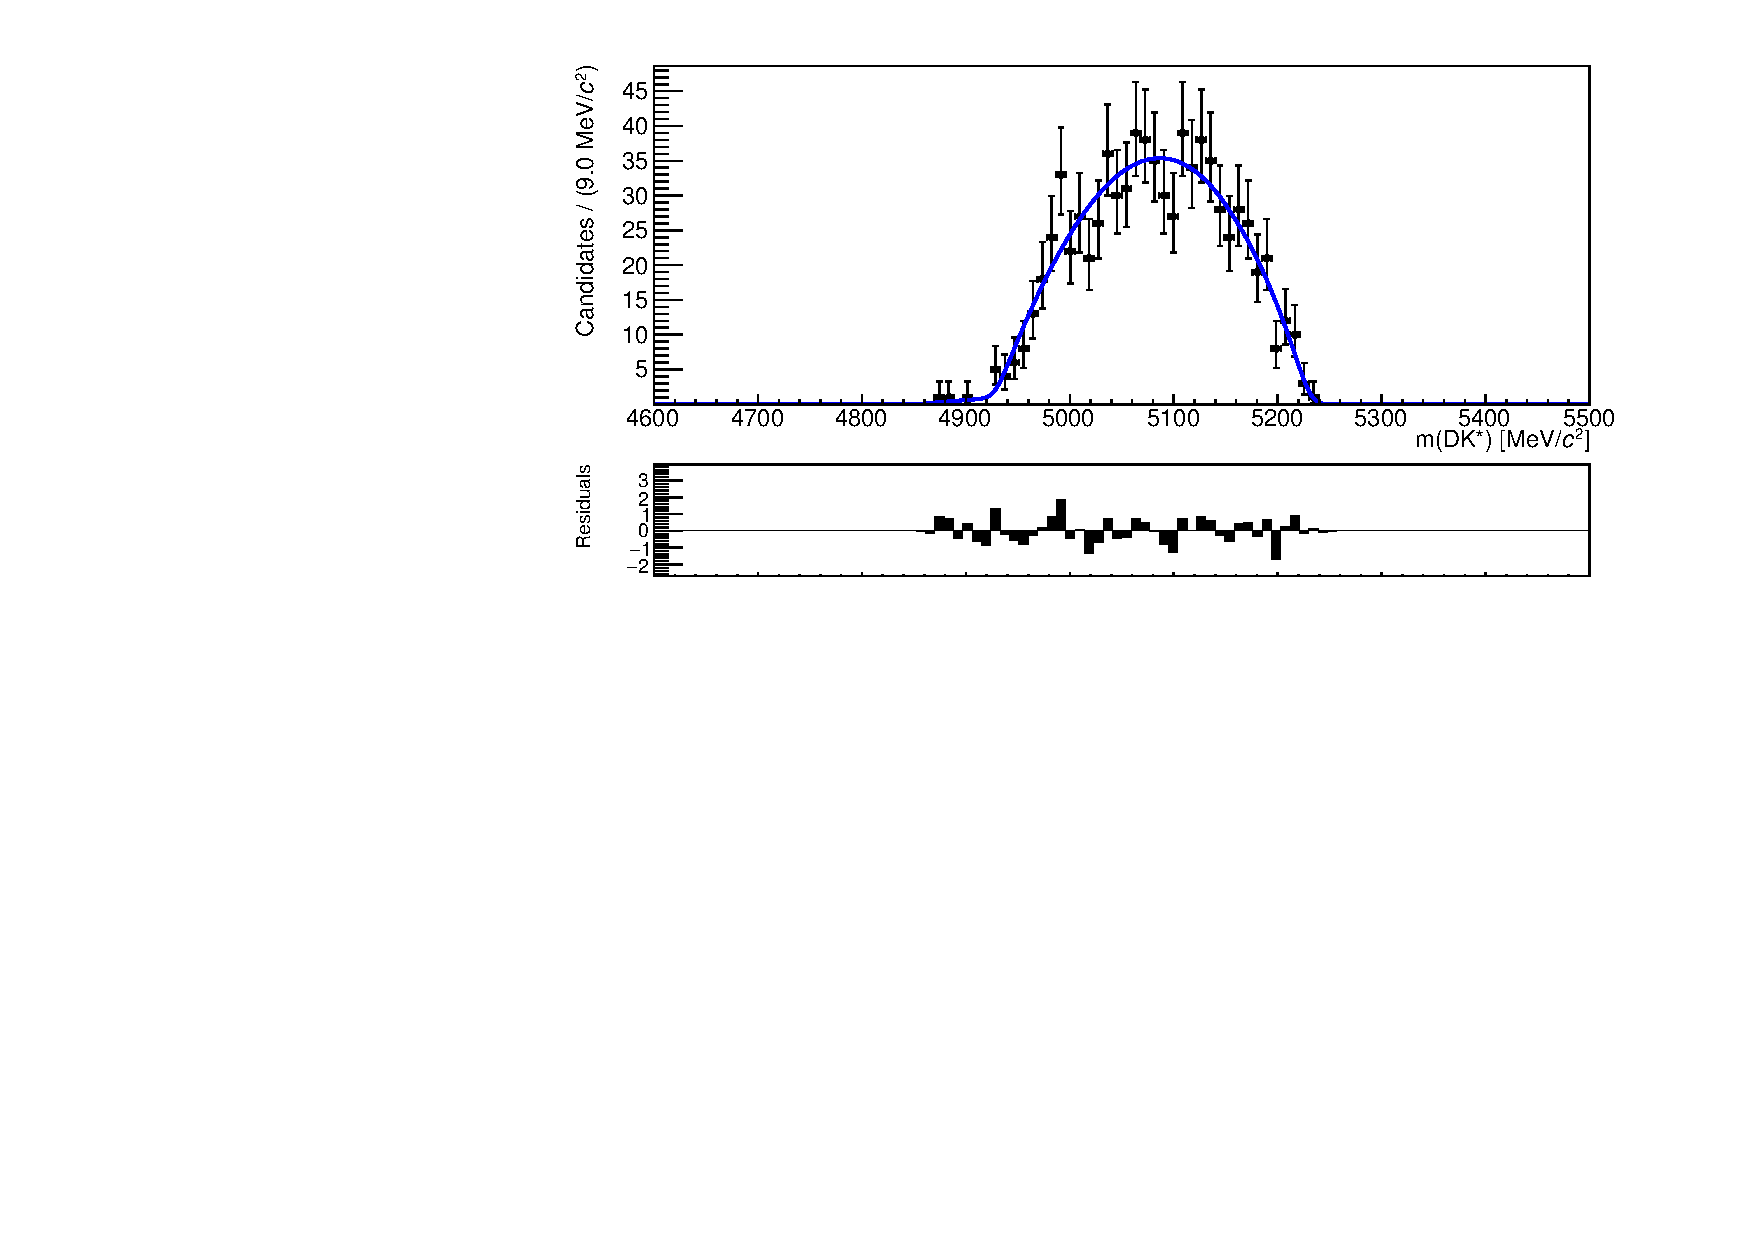
\includegraphics[width=0.5\linewidth]{figures/fitComponents/Bugamma010_LL.pdf}
\put(-180,80) {(c)}
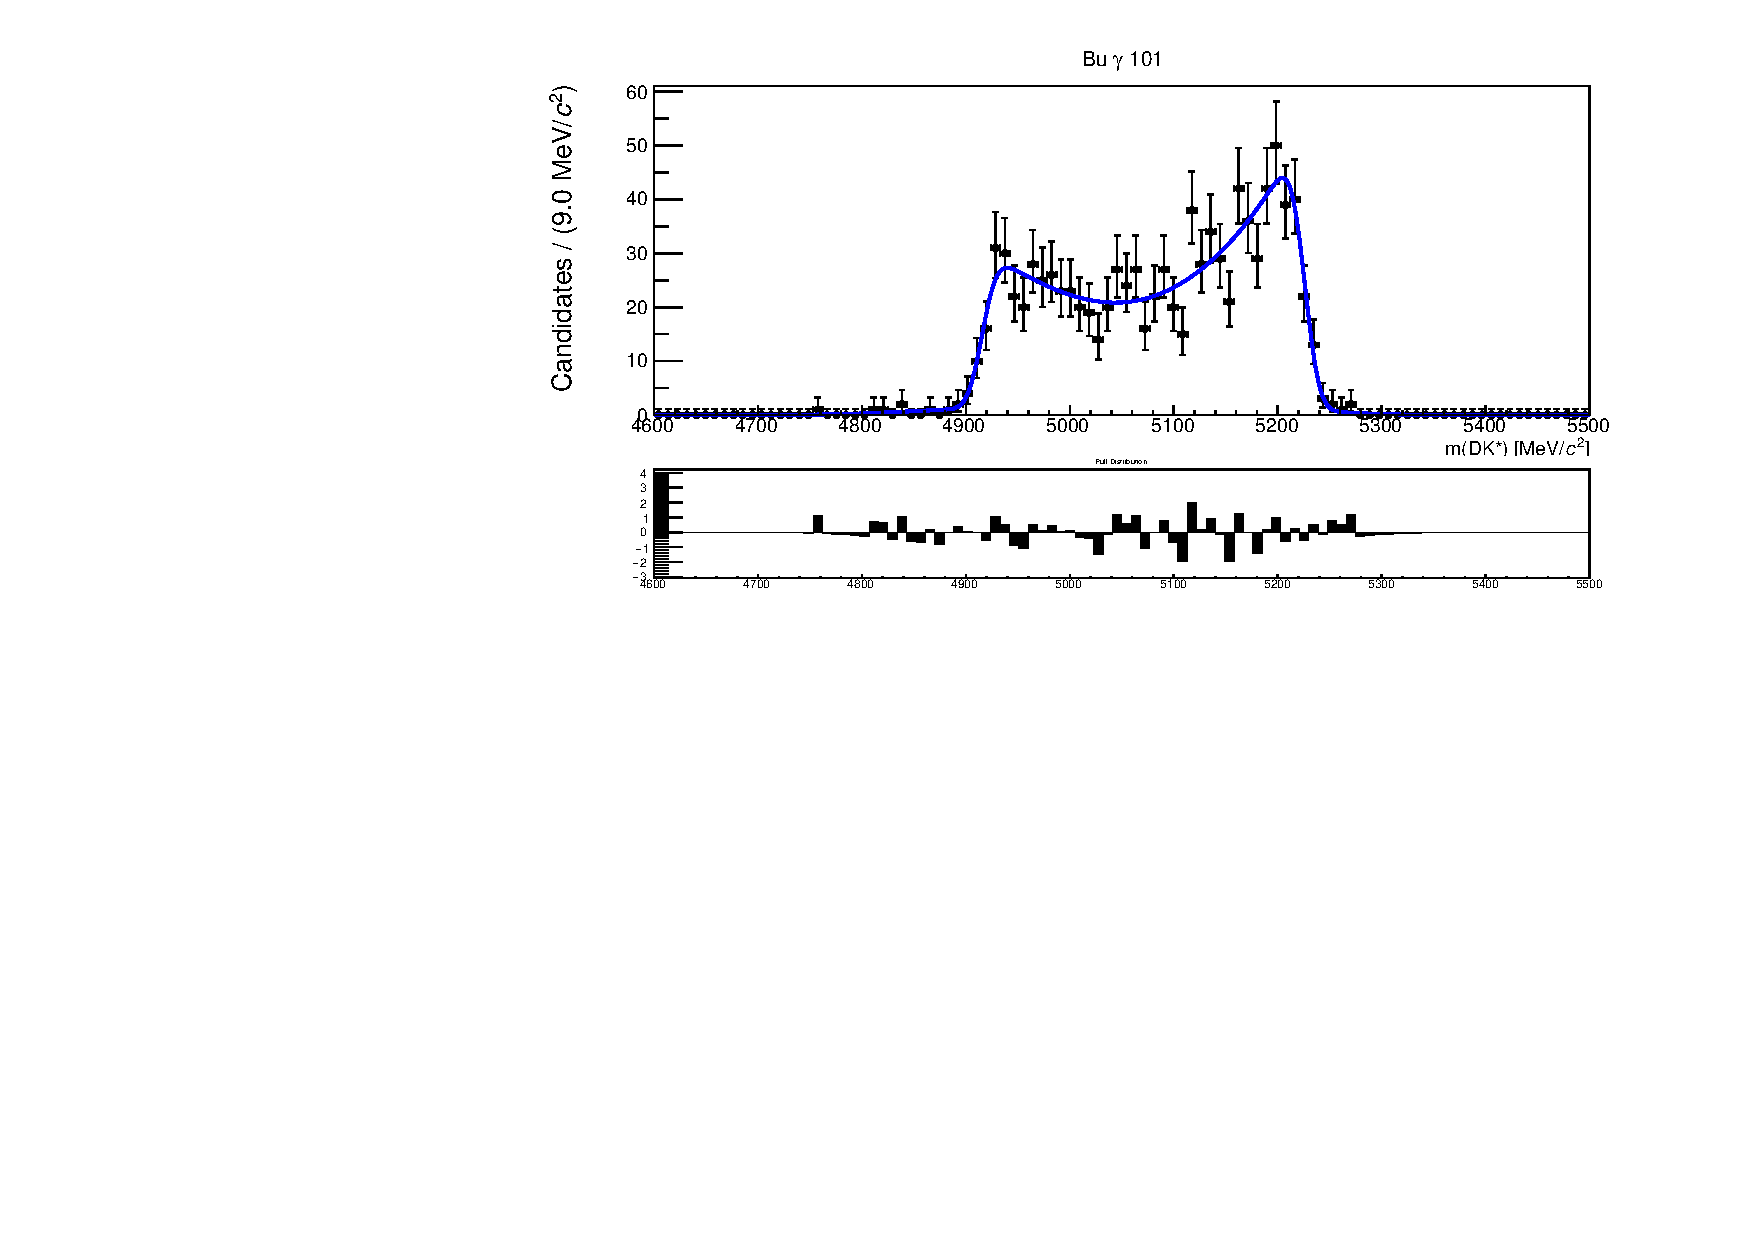
\includegraphics[width=0.5\linewidth]{figures/fitComponents/Bugamma101_LL.pdf}
\put(-180,80) {(d)}
\hfill
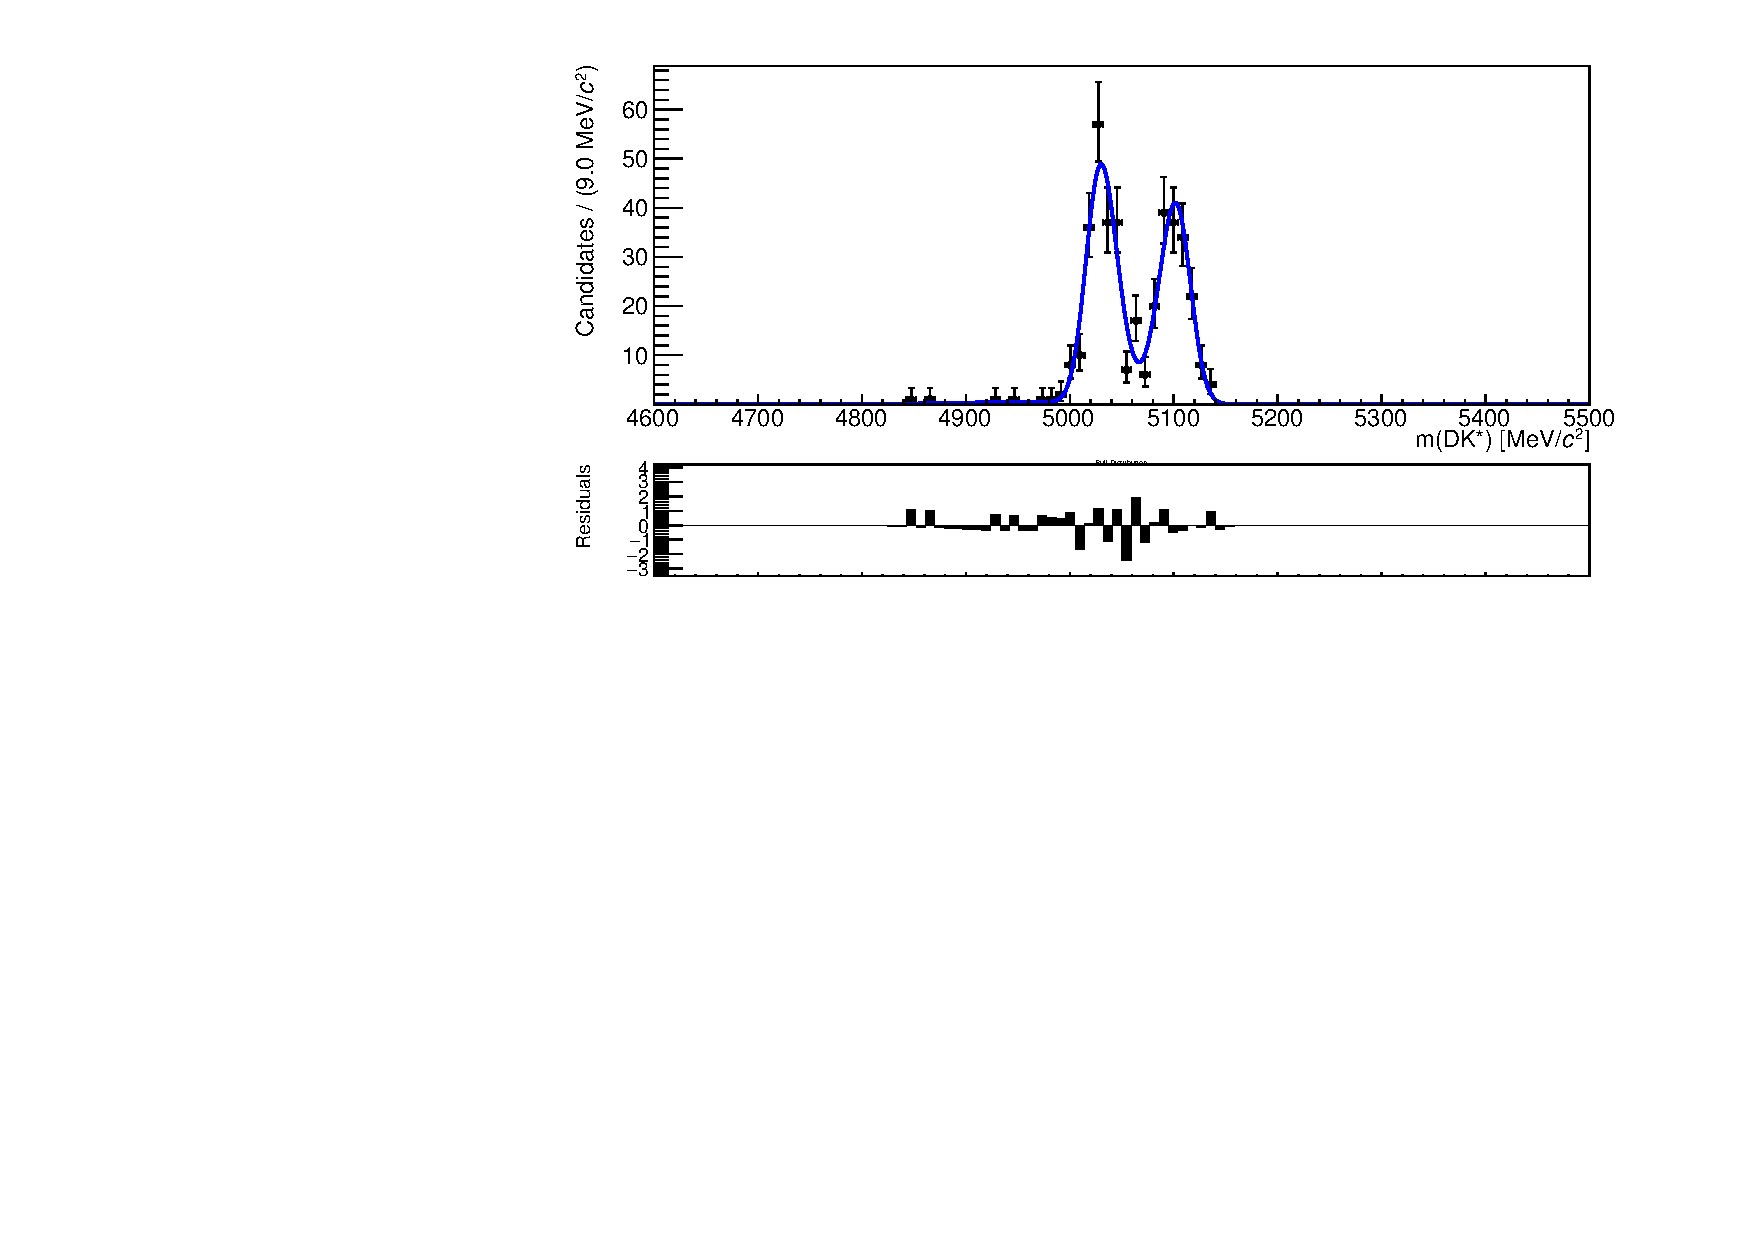
\includegraphics[width=0.5\linewidth]{figures/fitComponents/Bdpi010_LL.pdf}
\put(-180,80) {(e)}
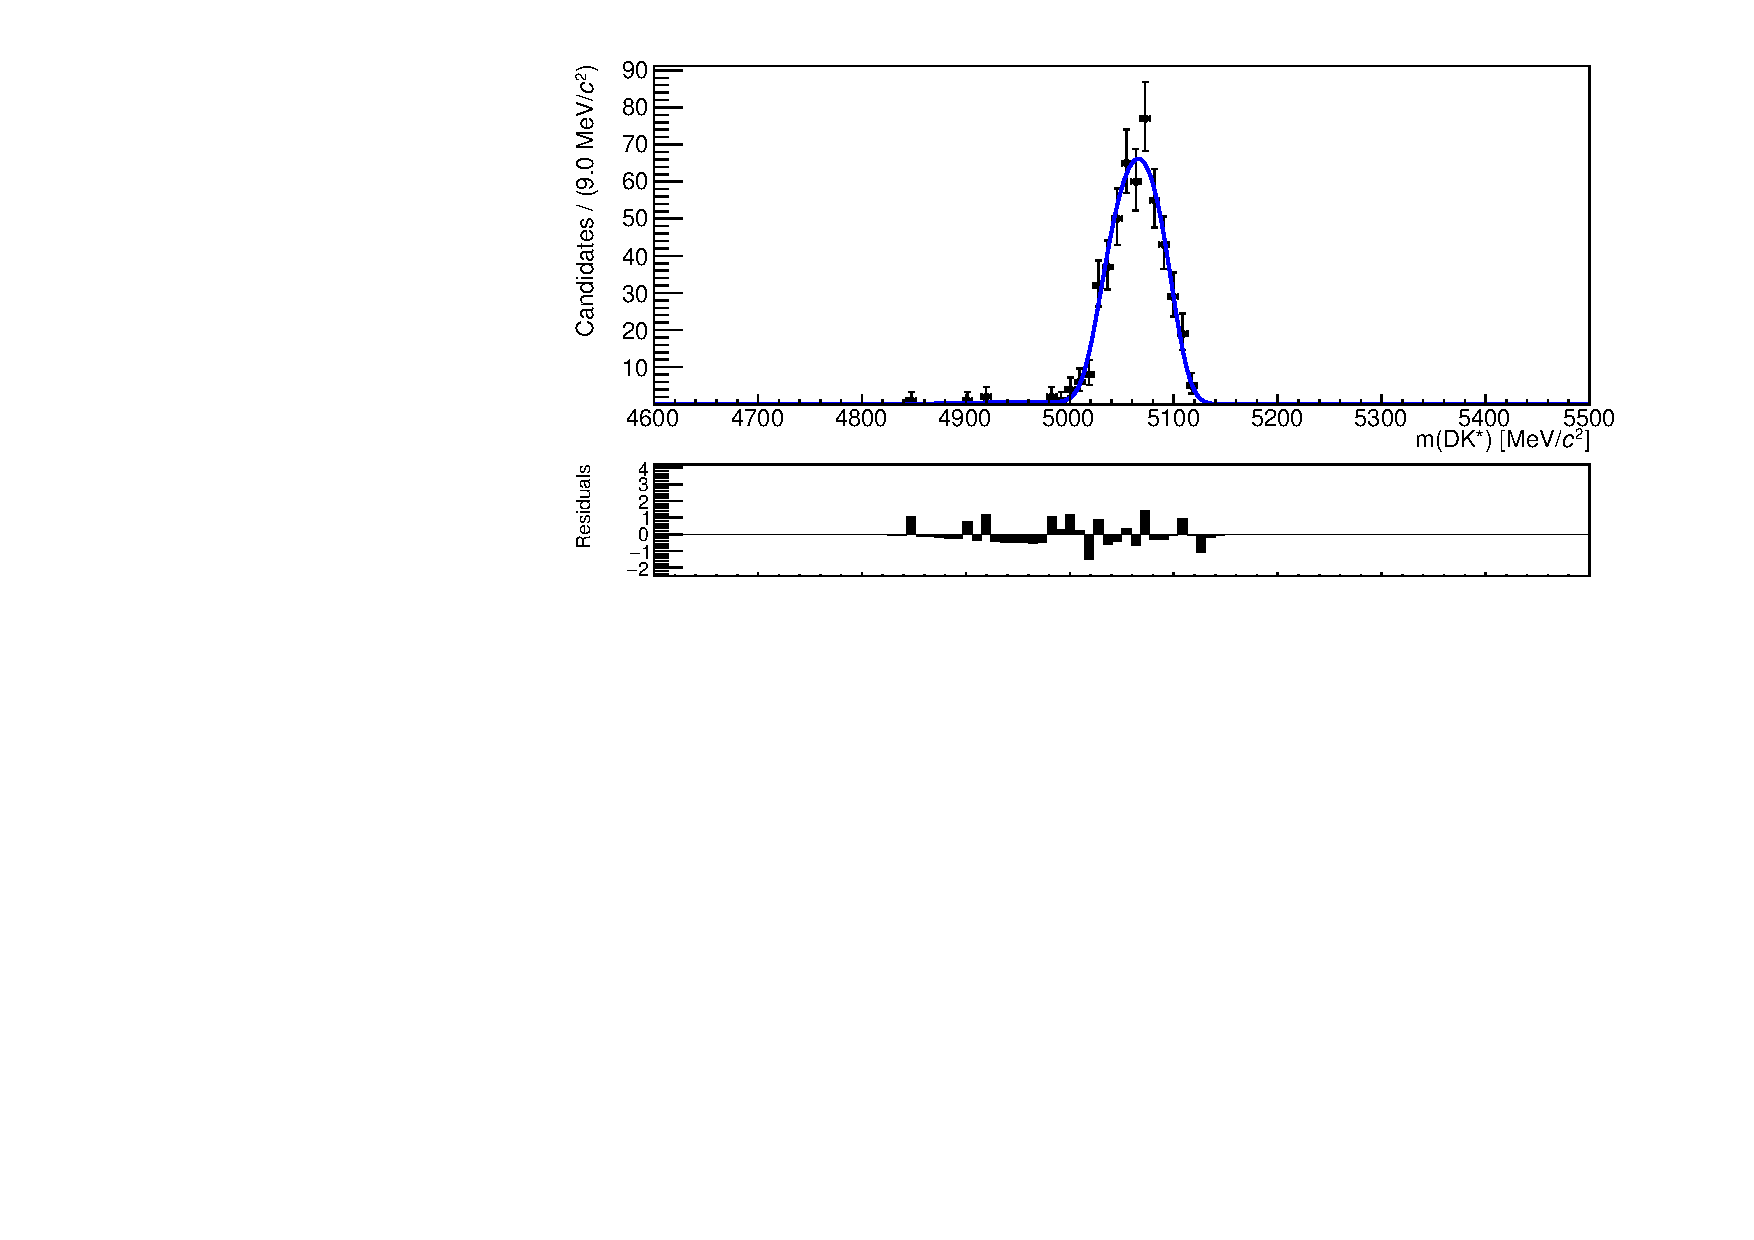
\includegraphics[width=0.5\linewidth]{figures/fitComponents/Bdpi101_LL.pdf}
\put(-180,80) {(f)}
\caption{Fit to $B \to D^*K^*$ Run 1 MC in all the different modes for LL candidates (a) \decay{\Bm}{(\decay{\Dstarz}{\Dz[\piz]})\Kstarm} 010, (b) \decay{\Bm}{(\decay{\Dstarz}{\Dz[\piz]})\Kstarm} 101, (c) \decay{\Bm}{(\decay{\Dstarz}{\Dz[\gamma]})\Kstarm} 010, (d) \decay{\Bm}{(\decay{\Dstarz}{\Dz[\gamma]})\Kstarm} 101, (e) \decay{\Bd}{(\decay{\Dstarp}{\Dz[\pip]})\Kstarm} 010, and (f) \decay{\Bd}{(\decay{\Dstarp}{\Dz[\pip]})\Kstarm} 101}
\label{partrecofitsLL}
\end{figure}

\begin{figure}
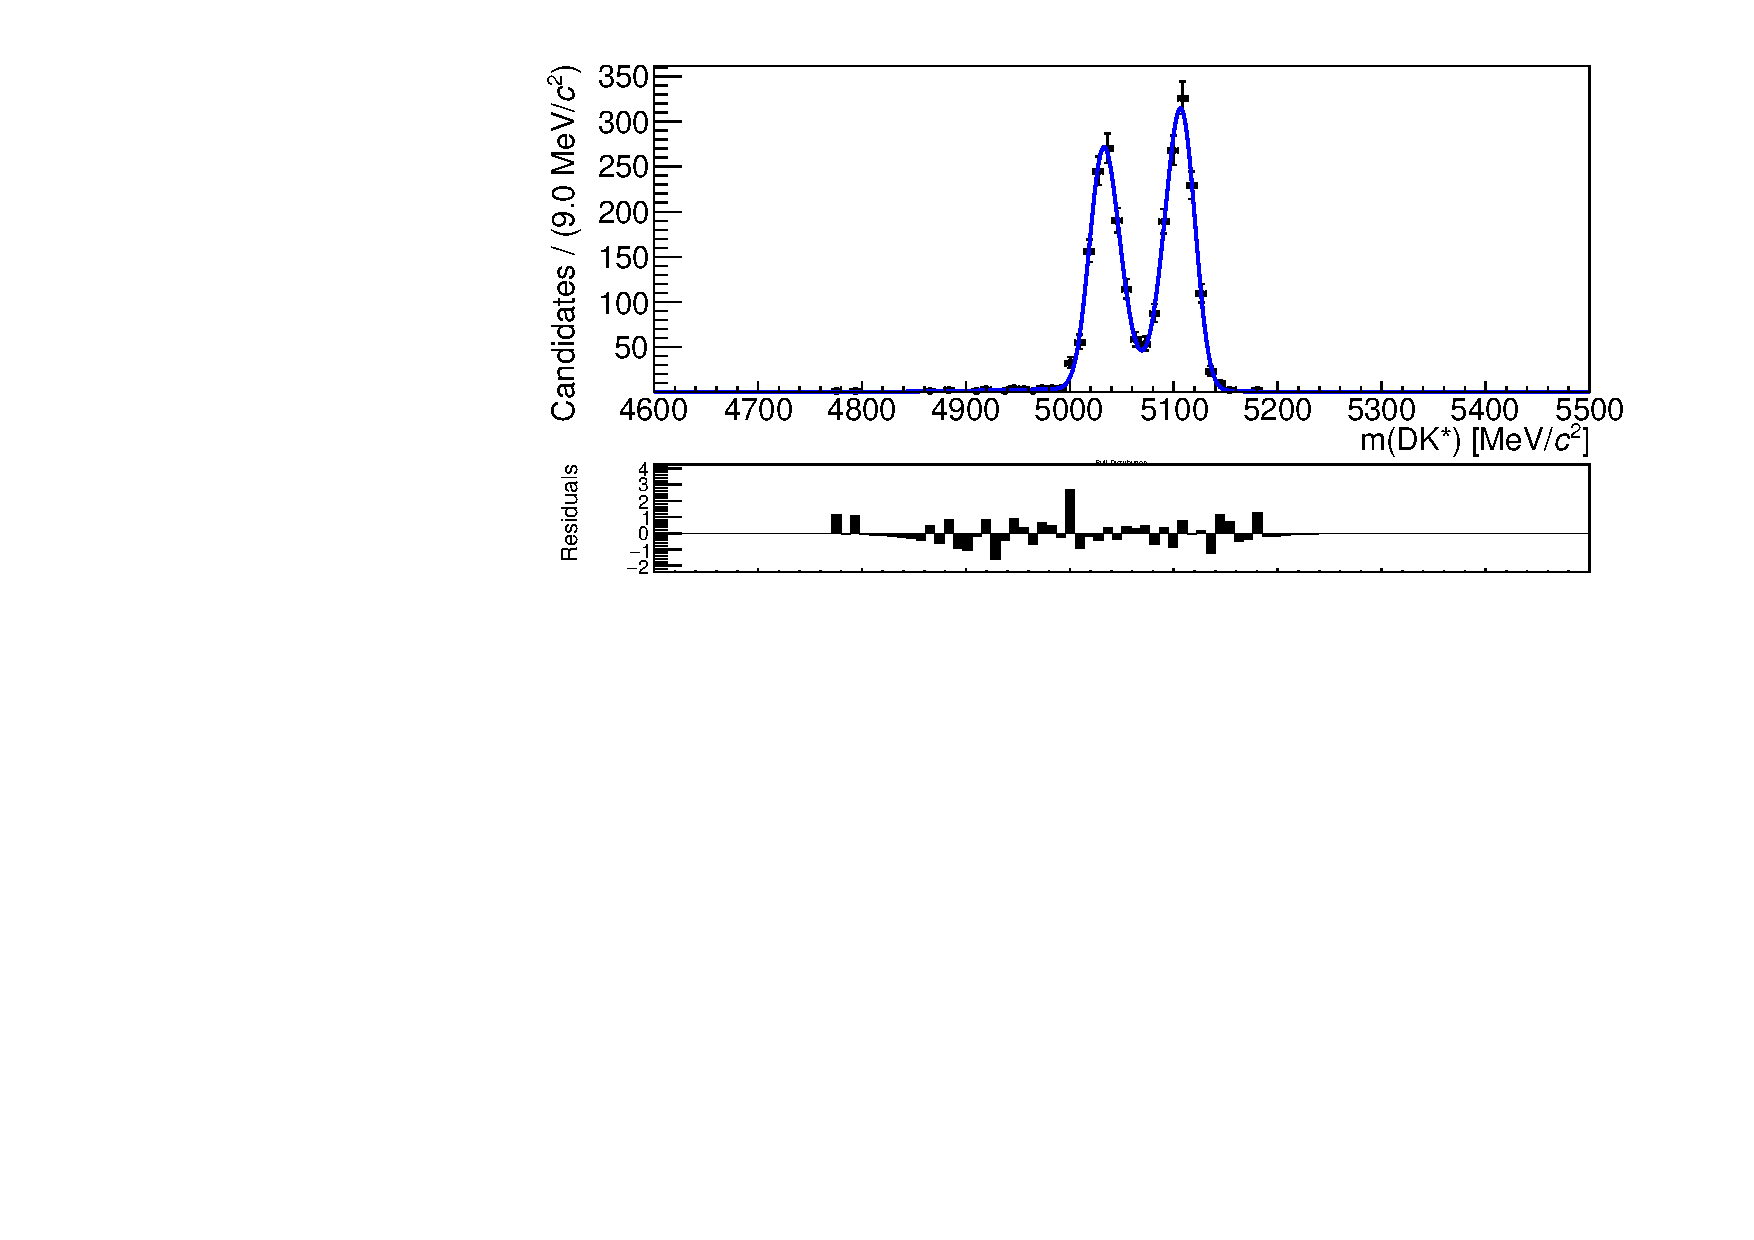
\includegraphics[width=0.5\linewidth]{figures/fitComponents/Bupi010_DD.pdf}
\put(-180,80) {(a)}
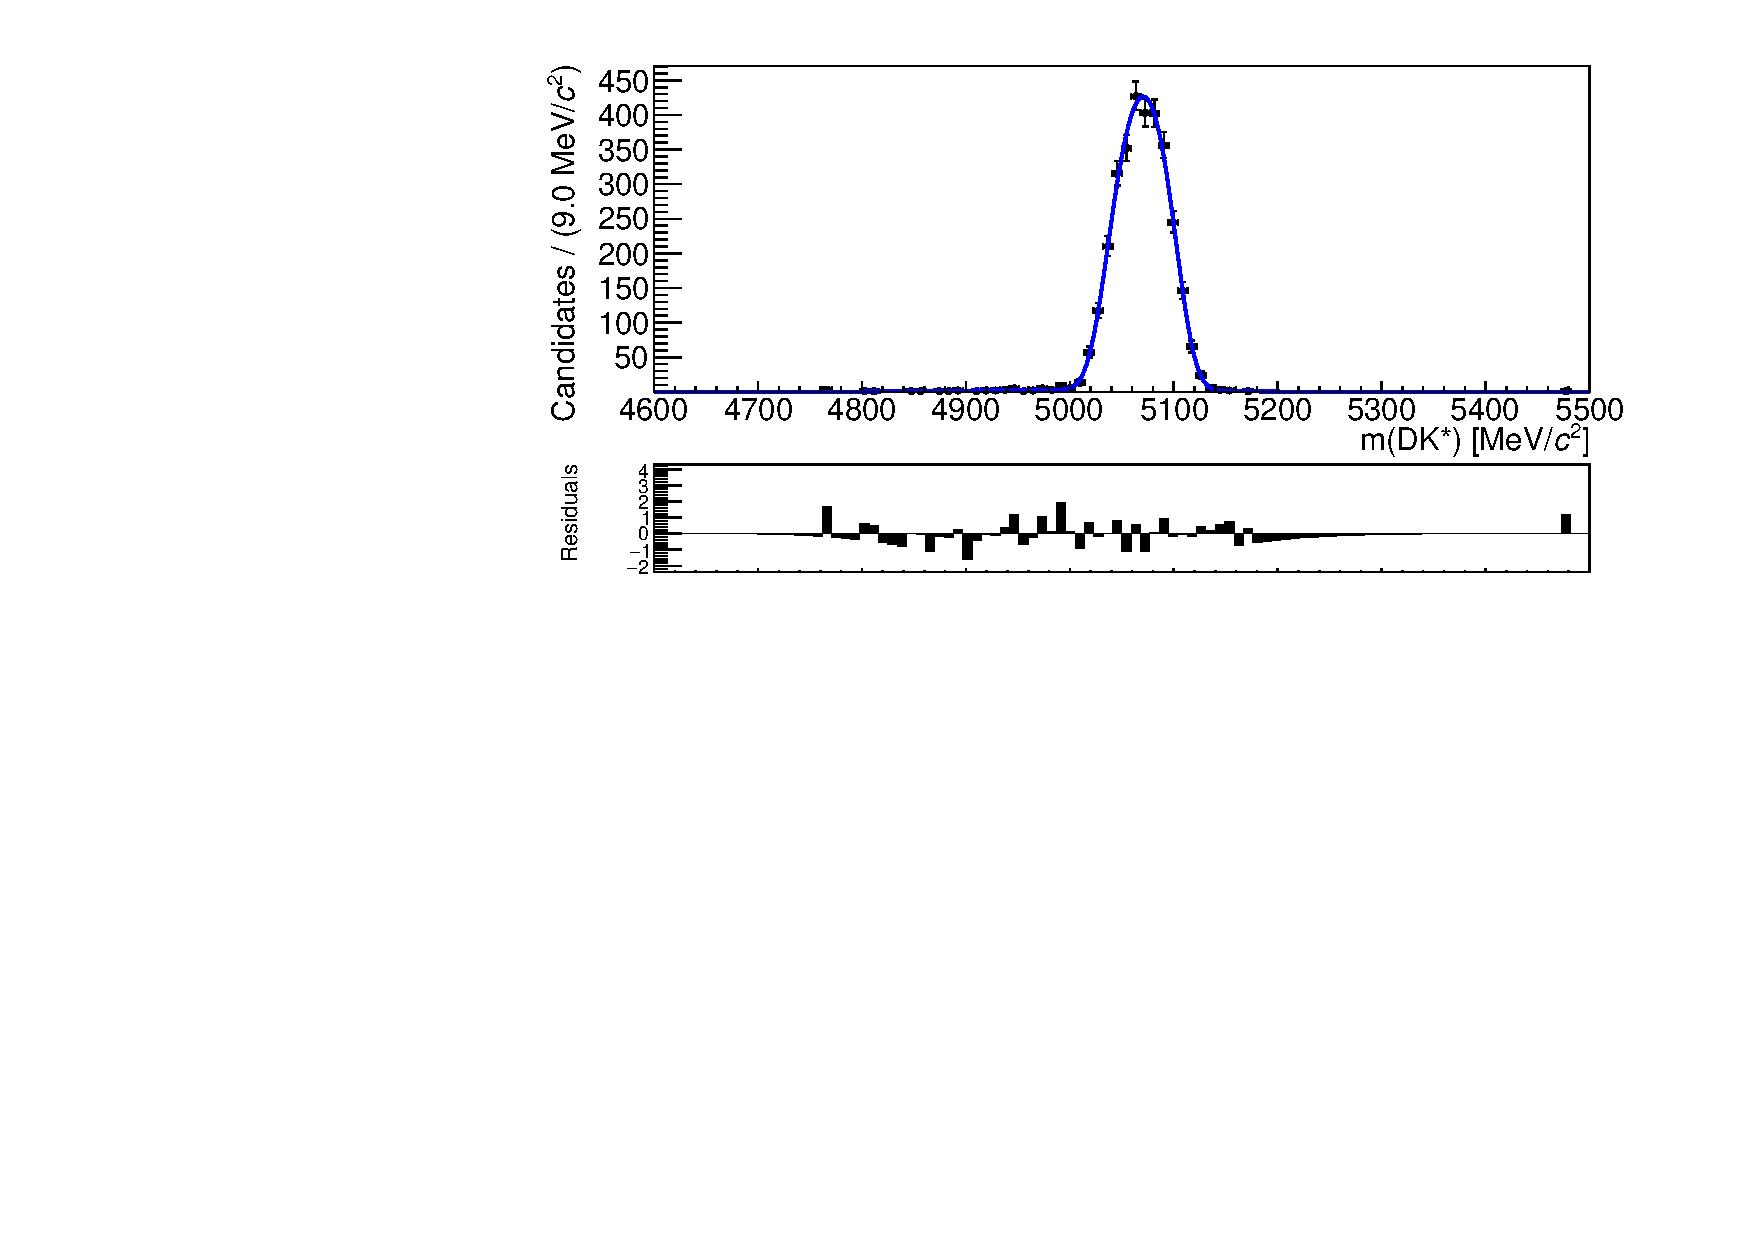
\includegraphics[width=0.5\linewidth]{figures/fitComponents/Bupi101_DD.pdf}
\put(-180,80) {(b)}
\hfill
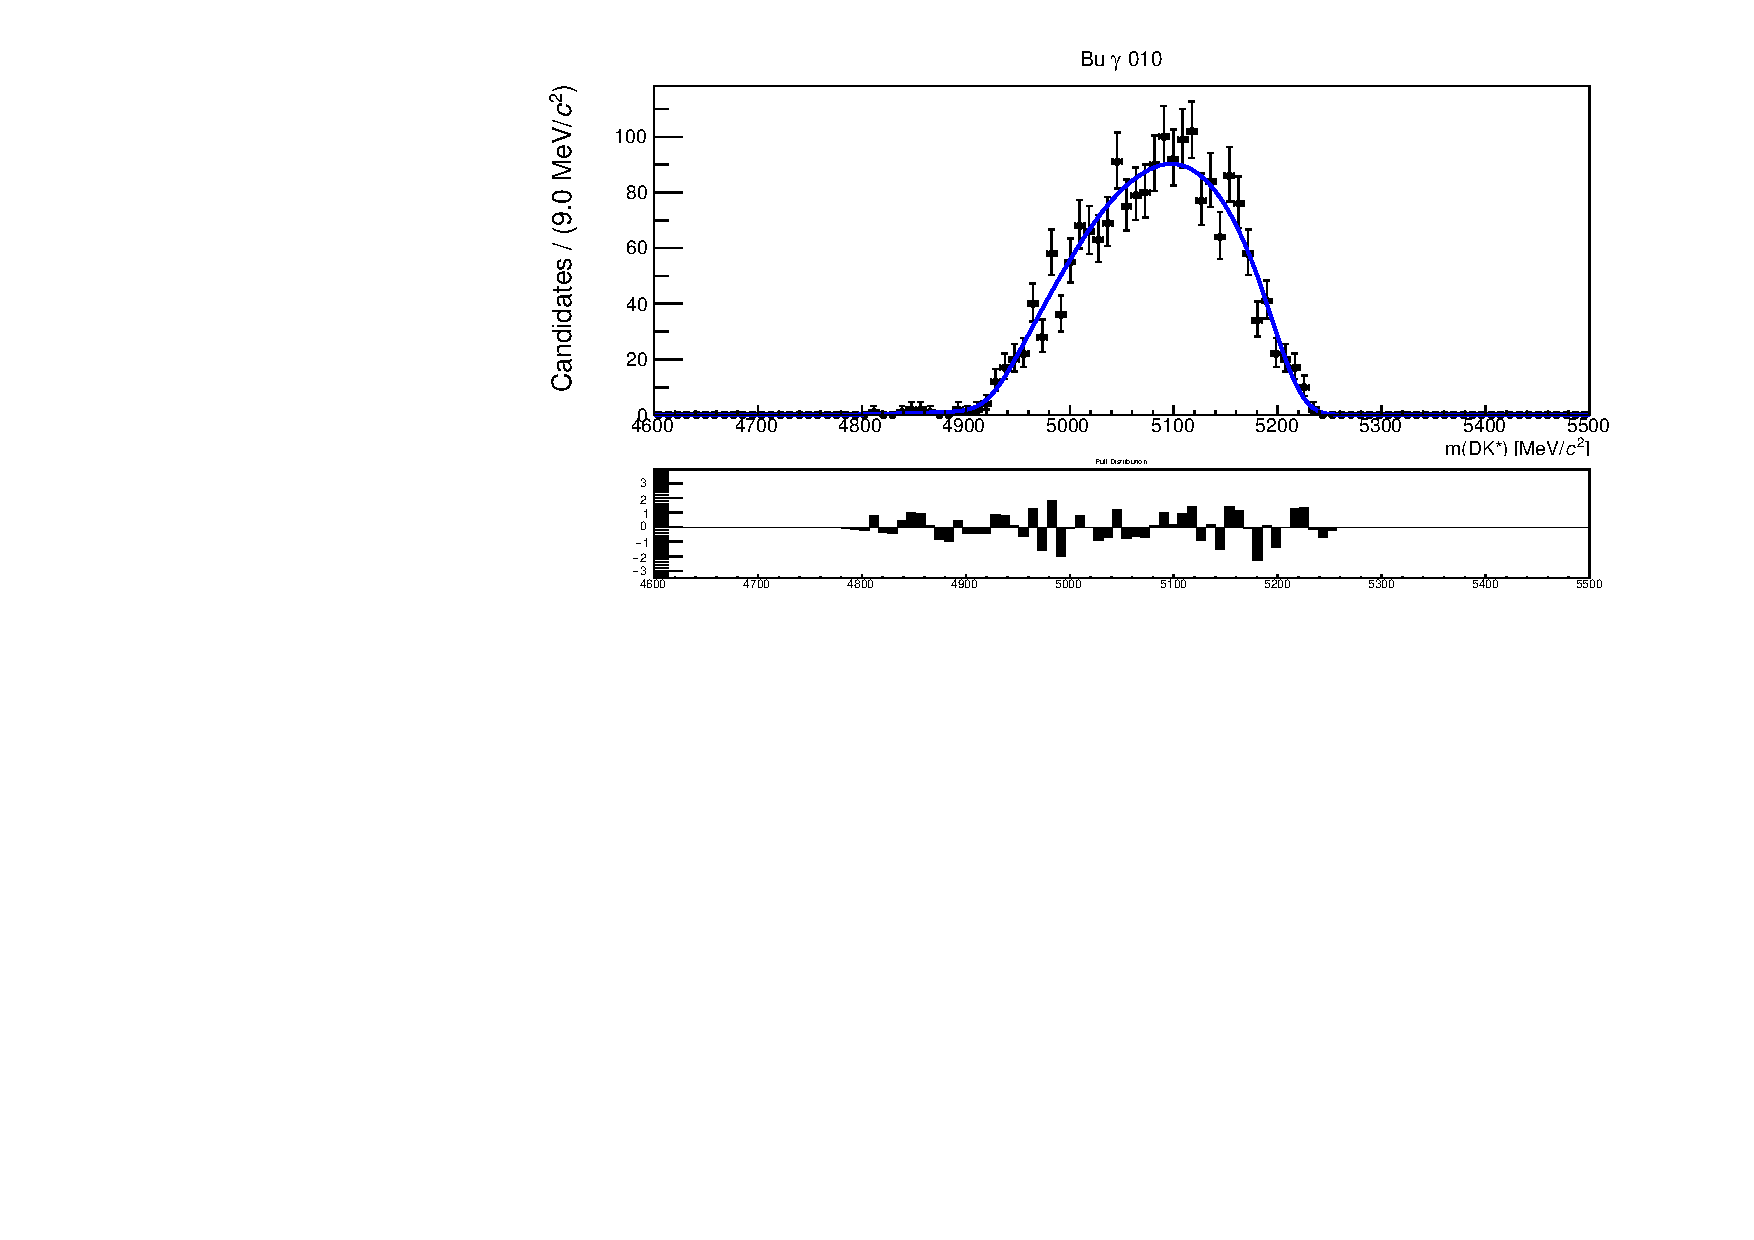
\includegraphics[width=0.5\linewidth]{figures/fitComponents/Bugamma010_DD.pdf}
\put(-180,80) {(c)}
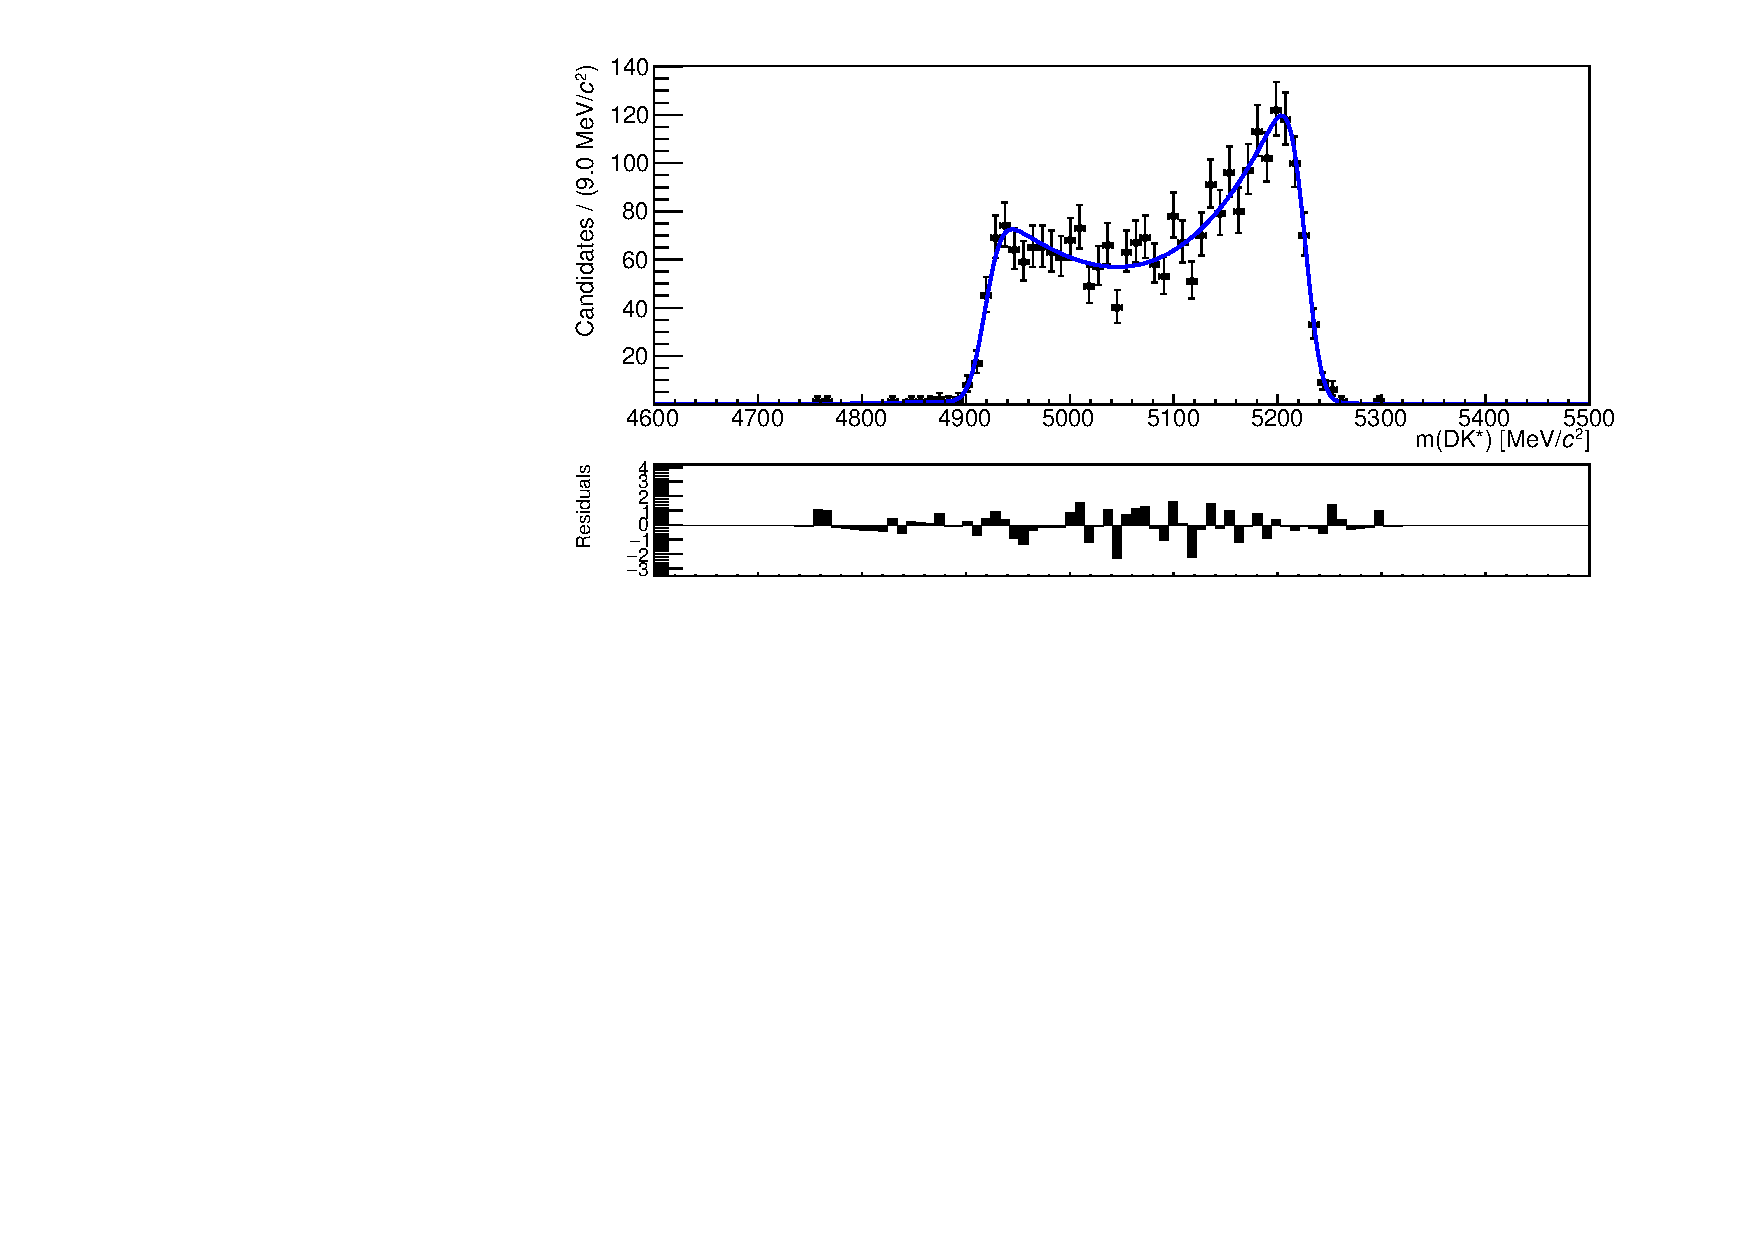
\includegraphics[width=0.5\linewidth]{figures/fitComponents/Bugamma101_DD.pdf}
\put(-180,80) {(d)}
\hfill
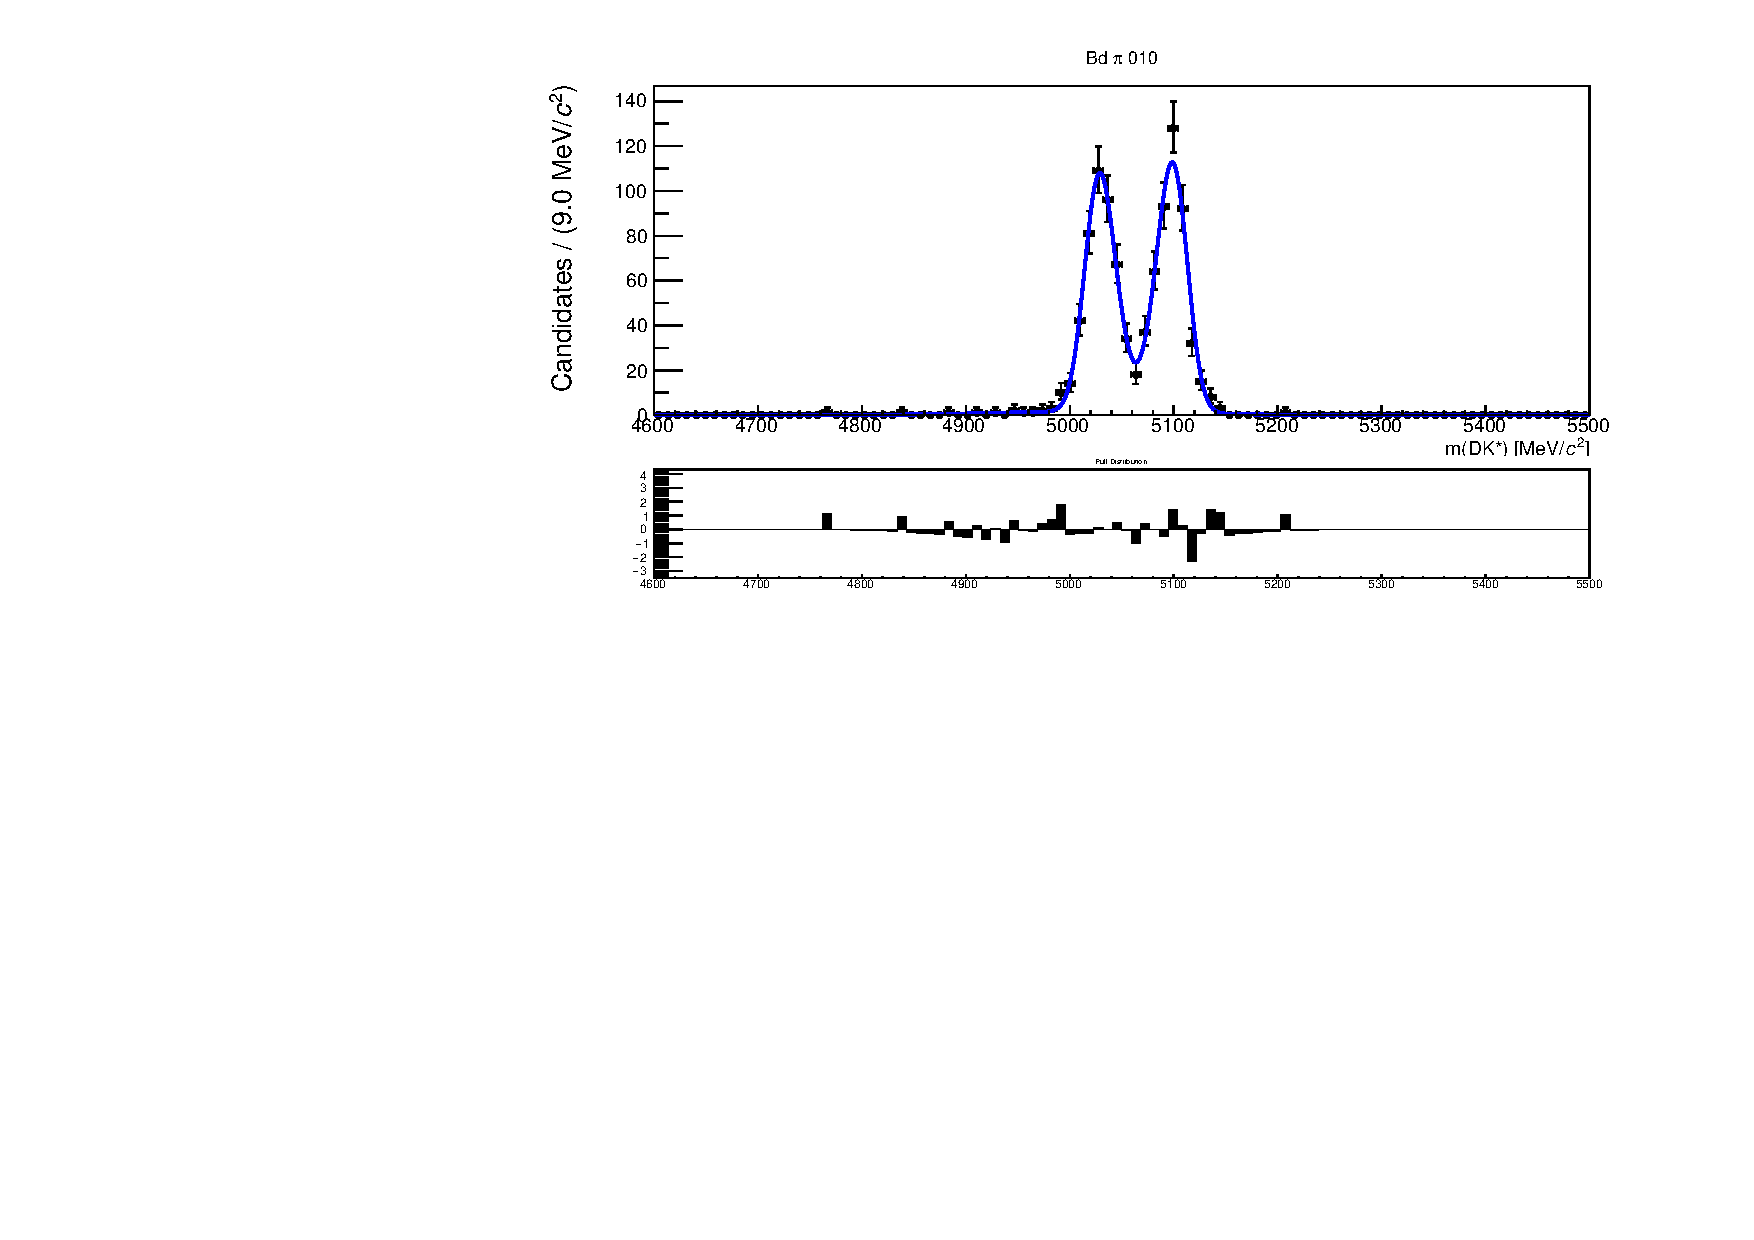
\includegraphics[width=0.5\linewidth]{figures/fitComponents/Bdpi010_DD.pdf}
\put(-180,80) {(e)}
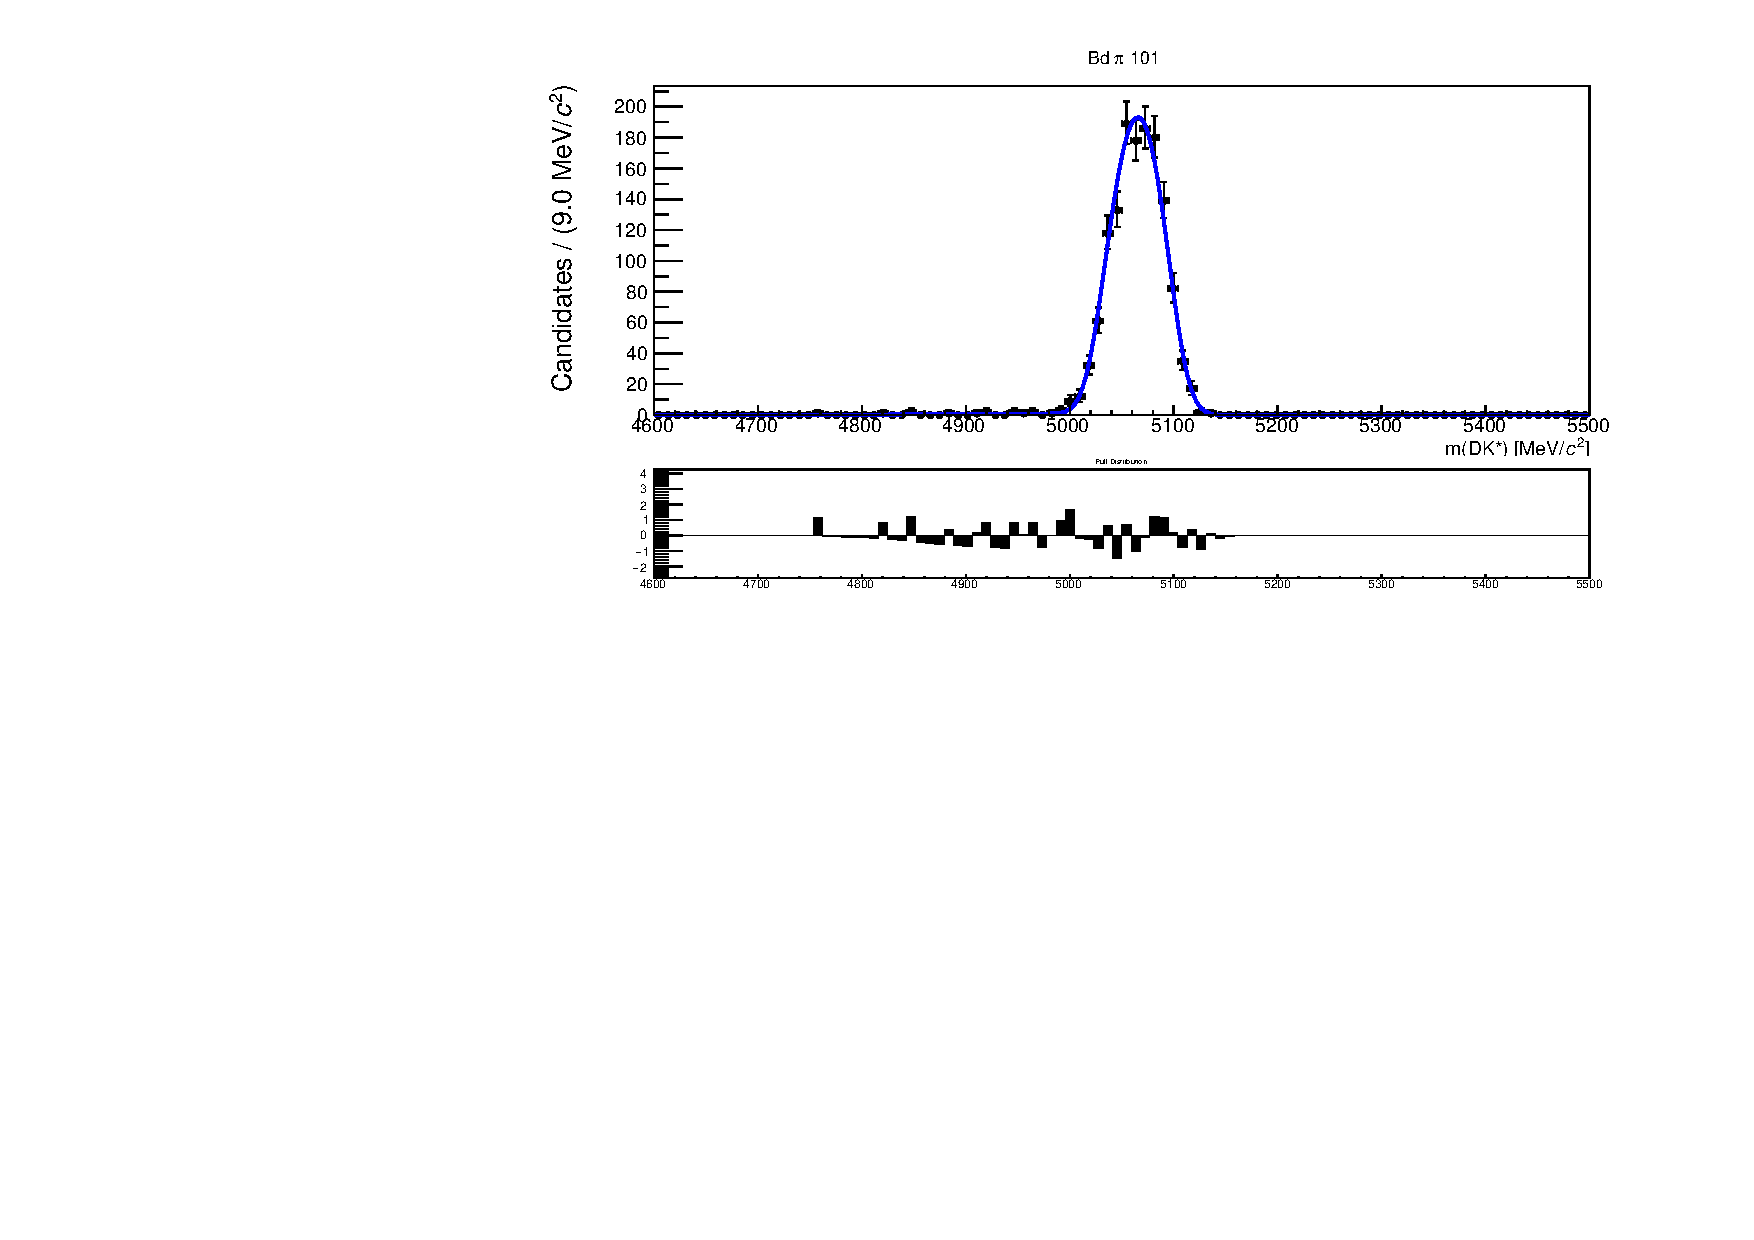
\includegraphics[width=0.5\linewidth]{figures/fitComponents/Bdpi101_DD.pdf}
\put(-180,80) {(f)}
\caption{Fit to $B \to D^*K^*$ Run 1 MC in all the different modes for DD candidates (a) \decay{\Bm}{(\decay{\Dstarz}{\Dz[\piz]})\Kstarm} 010, (b) \decay{\Bm}{(\decay{\Dstarz}{\Dz[\piz]})\Kstarm} 101, (c) \decay{\Bm}{(\decay{\Dstarz}{\Dz[\gamma]})\Kstarm} 010, (d) \decay{\Bm}{(\decay{\Dstarz}{\Dz[\gamma]})\Kstarm} 101, (e) \decay{\Bd}{(\decay{\Dstarp}{\Dz[\pip]})\Kstarm} 010, and (f) \decay{\Bd}{(\decay{\Dstarp}{\Dz[\pip]})\Kstarm} 101}
\label{partrecofitsDD}
\end{figure}

As there are six shapes in this low mass region of the mass fit, from 4900-5230 MeV, it is necessary to fix some yields in order to have a stable fit. The yield ratios between \decay{\Bm}{(\decay{\Dstarz}{\Dz[\piz]})\Kstarm}, \decay{\Bm}{(\decay{\Dstarz}{\Dz[\gamma]})\Kstarm} and \decay{\Bd}{(\decay{\Dstarp}{\Dz[\pip]})\Kstarm} are fixed separately for the 010 and 101 helicity amplitudes. The values fixed in the fit, given in Table \ref{fixedyieldratios}, are obtained from a ratio of braching fractions and selection efficiencies, an example calculation is given in Equation \ref{partrecoexample}. This calculation is performed for each of the ratios listed in Table \ref{fixedyieldratios}. Branching fractions for the partially reconstructed decays are given in Table \ref{partrecoBRs}. MC events are generated for each of the modes and the values of $\epsilon_{sel}$, used in Equation \ref{partrecoexample}, are given by the fraction of MC events passing the selection.

\begin{equation}
\frac{N(\decay{\B}{(\decay{\Dstar}{\Dz\piz})\Kstar}\ 010)}{N(\decay{\B}{(\decay{\Dstar}{\Dz\gamma})\Kstar}\ 010)} = \frac{BR(\decay{\B}{(\decay{\Dstar}{\Dz\piz})\Kstar})}{BR(\decay{\B}{(\decay{\Dstar}{\Dz\gamma})\Kstar})} \times \frac{\epsilon_{sel}(\decay{\B}{(\decay{\Dstar}{\Dz\piz})\Kstar}\ 010)}{\epsilon_{sel}(\decay{\B}{(\decay{\Dstar}{\Dz\gamma})\Kstar}\ 010)}
\label{partrecoexample}
\end{equation}

\begin{table}[h]
\centering
\begin{tabular}{c|c}
Mode & Branching ratio \\
\hline
\decay{\Bm}{(\decay{\Dstarz}{\Dz[\piz]})\Kstarm} & $(5.0 \pm 0.9) \times 10^{-4}$ \\
\decay{\Bm}{(\decay{\Dstarz}{\Dz[\gamma]})\Kstarm} & $(3.1 \pm 0.6) \times 10^{-4}$ \\
\decay{\Bd}{(\decay{\Dstarp}{\Dz[\pip]})\Kstarm} & $(2.2 \pm 0.4) \times 10^{-4}$ \\
\end{tabular}
\caption{Branching ratios for the different partially reconstructed decay modes~\cite{PDG2014}}
\label{partrecoBRs}
\end{table}

\begin{table}
\centering
\begin{tabular}{ccc}
\hline
& LL & DD \\
\hline
$\frac{Bu \gamma 010}{Bu \pi 010}$ & $0.53 \pm 0.14$ & $0.51 \pm 0.14$ \\[3mm]
$\frac{Bd \pi 010}{Bu \pi 010}$ & $0.38 \pm 0.14$ & $0.37 \pm 0.14$ \\[3mm]
$\frac{Bu \gamma 101}{Bu \pi 101}$ & $0.53 \pm 0.14$ & $0.51 \pm 0.14$ \\[3mm]
$\frac{Bd \pi 101}{Bu \pi 101}$ & $0.38 \pm 0.14$ & $0.38 \pm 0.14$ \\[3mm]
\hline
\end{tabular}
\caption{Yield ratios fixed in the mass fit for the partically reconstructed backgrounds}
\label{fixedyieldratios}
\end{table}

Other backgrounds investigated in this analysis, but not included in the mass fit are discussed in Section \ref{sec:backgrounds}.


\subsection{Mass fit}
\label{sec:massfit:fit}

A fit to the invariant B mass in the $K\pi$ and $K\pi\pi\pi$ favoured mode is performed using the shapes discussed in Sections \ref{sec:massfit:signal}, \ref{sec:massfit:combinatorial} and \ref{sec:massfit:partreco}. The yield of the signal and combinatoric shape are left to float without constraint. There are six shapes in the partially reconstructed background. The yield ratios between all the shapes with helicity amplitude 010 and yield ratios between the shapes with helicity amplitude 101 are fixed to the values detailed in Table \ref{fixedyieldratios}. The only parameters left floating in the partially reconstructed background are the yield ratio between the 010 and 101 amplitudes and the overall yield. 

Figures \ref{massfitskpi} and \ref{massfitsk3pi} shows the fits to the invariant B mass distribution in the $K\pi$ and $K\pi\pi\pi$ favoured mode respectively for LL and DD candidates in both Run 1 and Run 2. The estimated $K\pi$ signal yield extracted from these fits for Run 1 is $220 \pm 16$ for LL and $505 \pm 24$ for DD, and for Run 2 is $388 \pm 21$ for LL and $901 \pm 33$ for DD. The fit results are shown in Table \ref{fitresultskpi}. For the $K\pi\pi\pi$ mode, the estimated signal yield extracted from these fits for Run 1 is $87 \pm 10$ for LL and $205 \pm 16$ for DD, and for Run 2 is $215 \pm 15$ for LL and $516 \pm 25$ for DD. The fit results are shown in Table \ref{fitresultsk3pi}.

\begin{figure}
\centering
\subfloat[Run 1 LL]{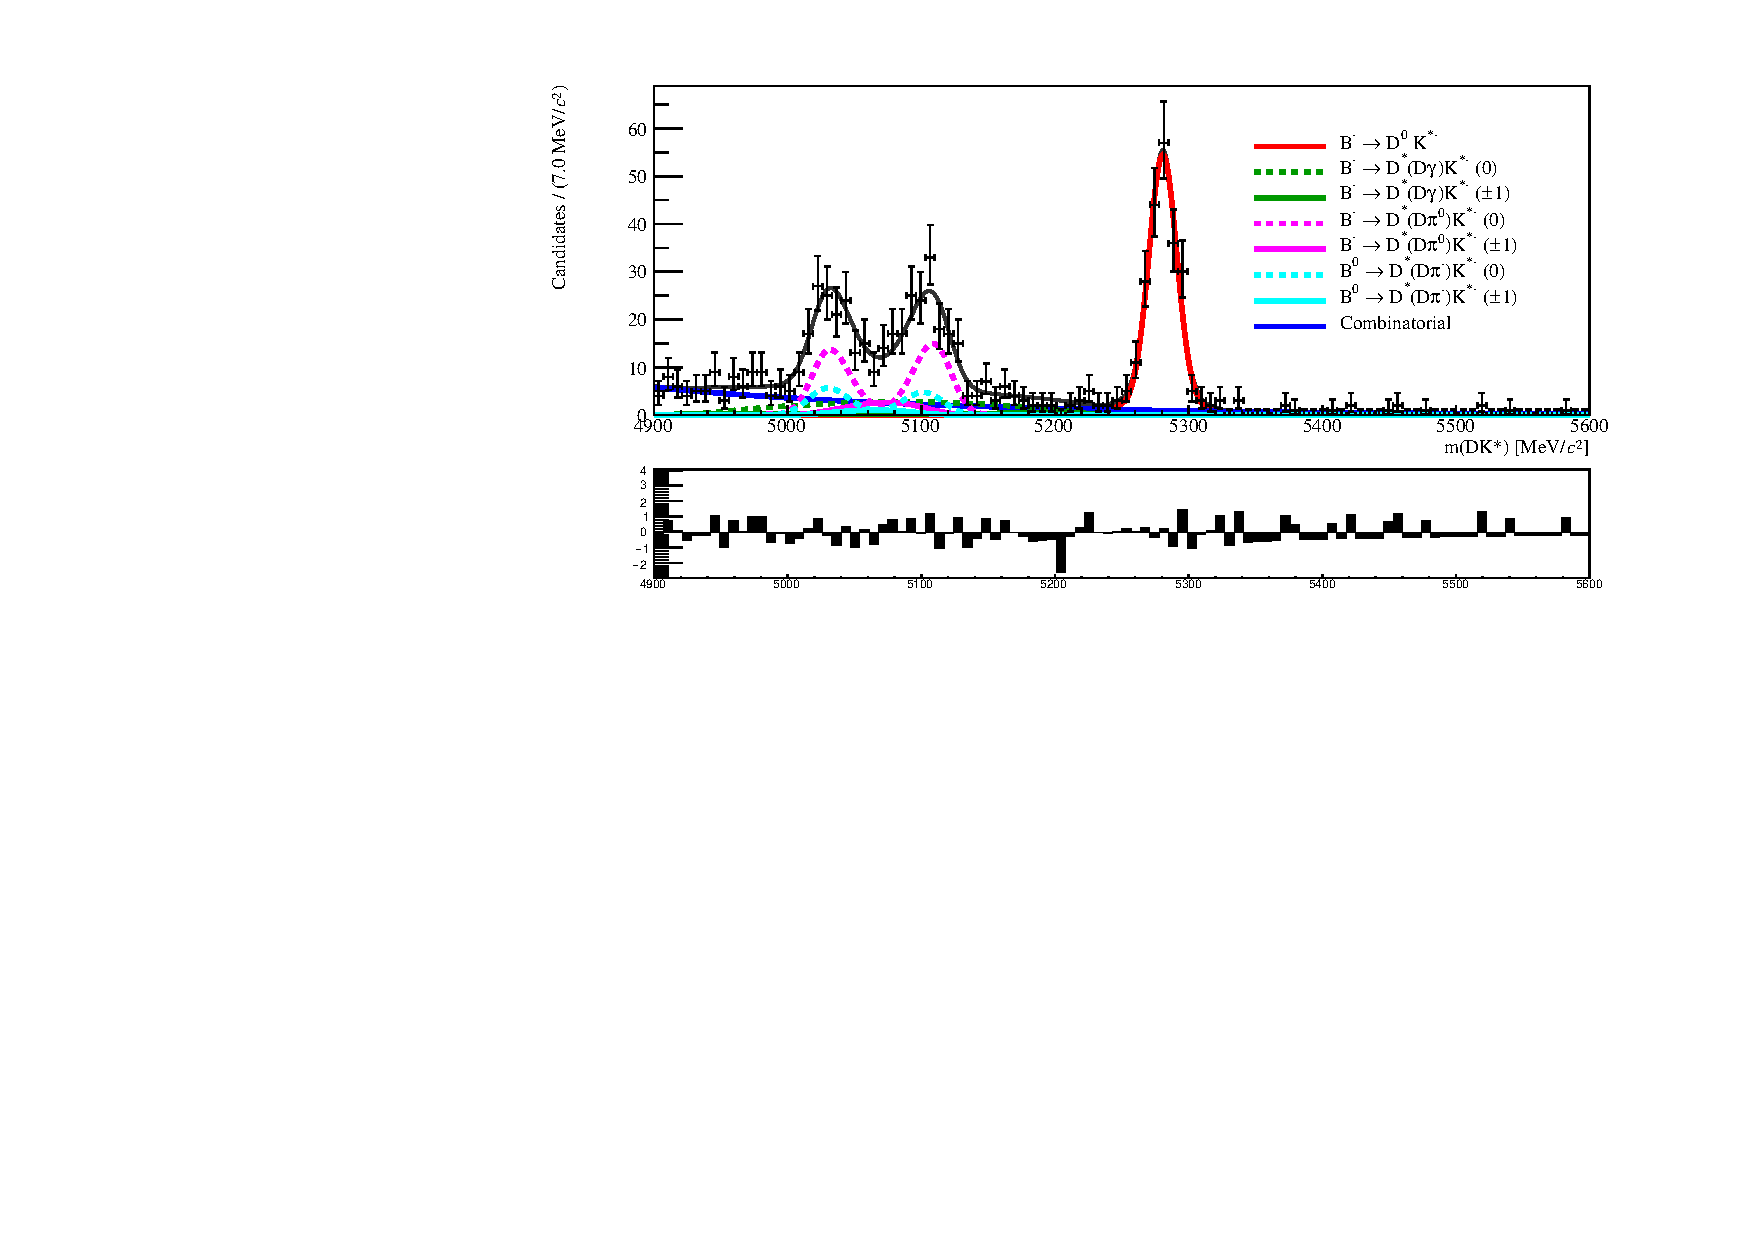
\includegraphics[width=0.7\linewidth]{figures/fitComponents/massFit_LL_KPi_run1.pdf}}
\vspace{-12pt}
\hfill
\subfloat[Run 1 DD]{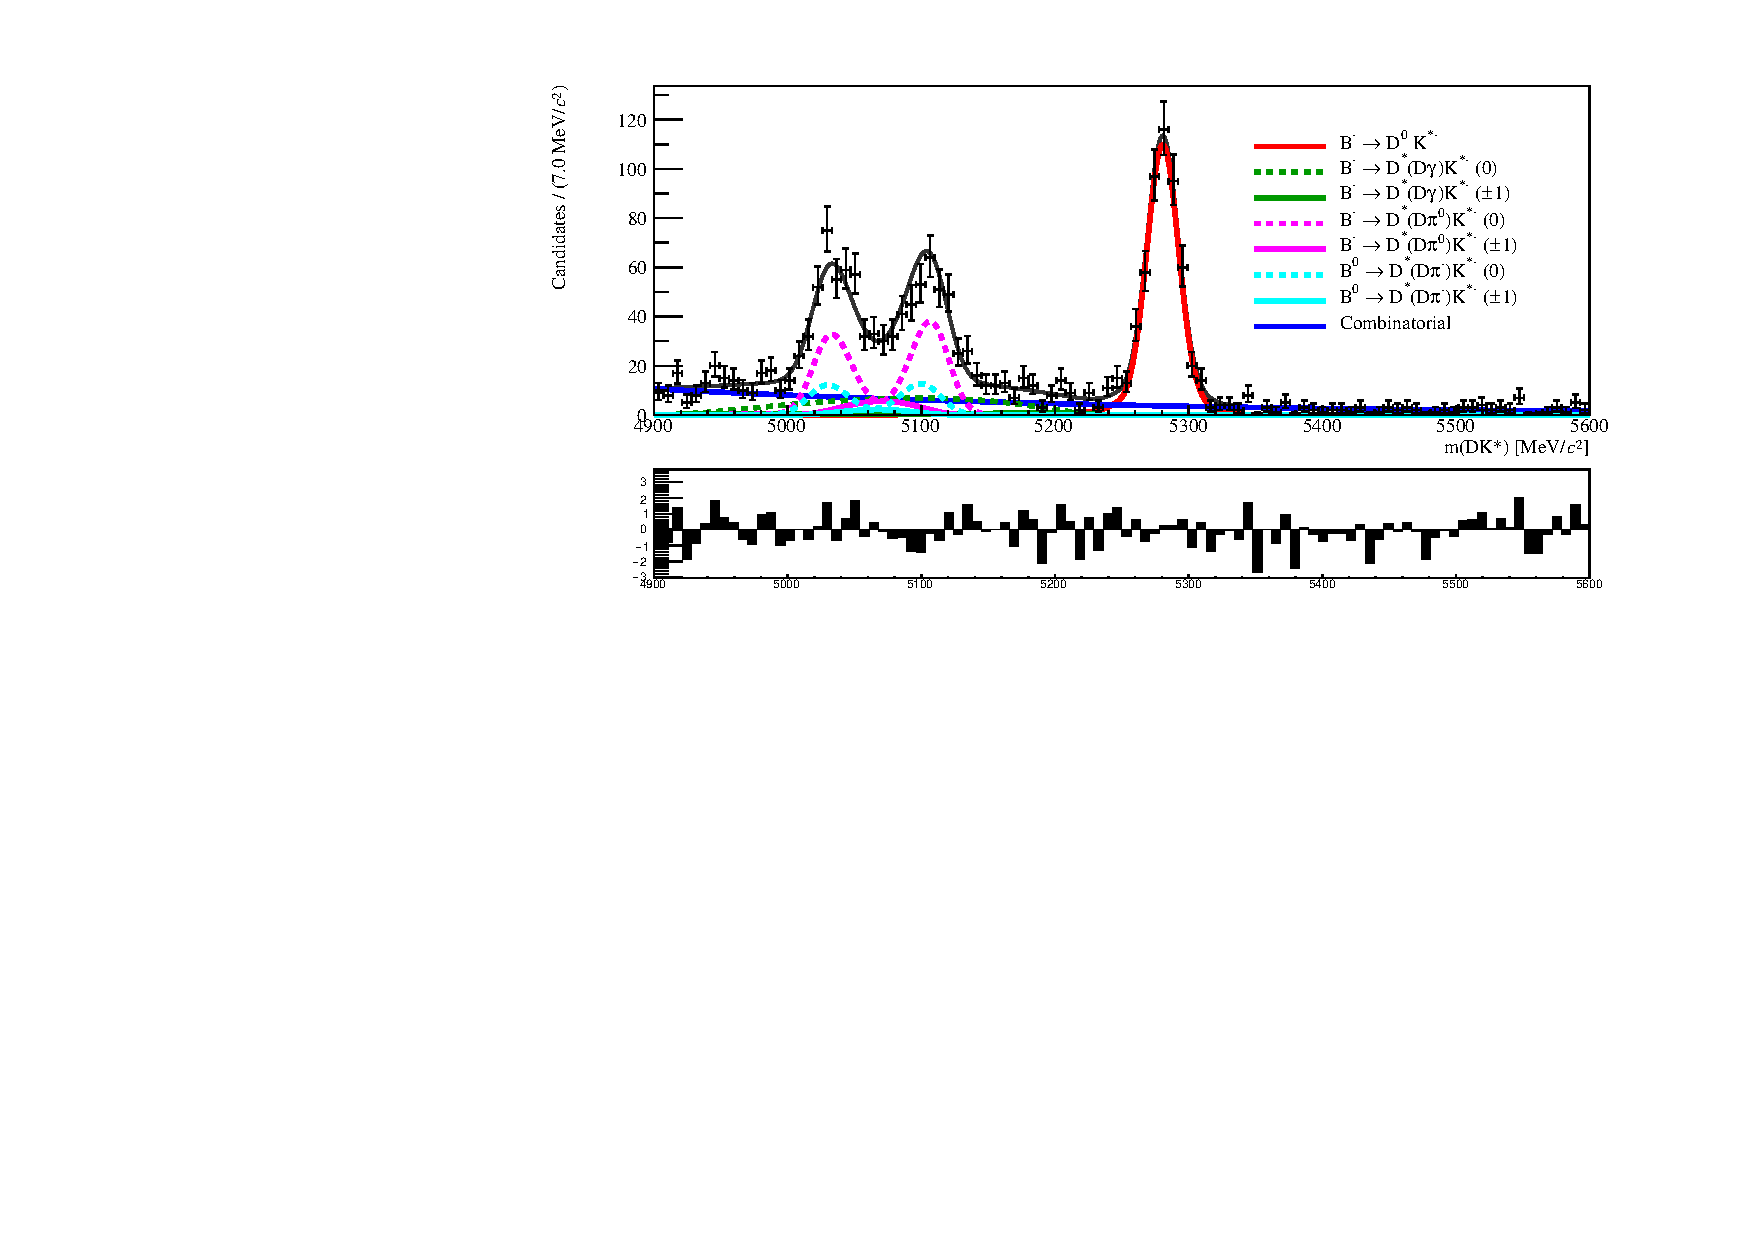
\includegraphics[width=0.7\linewidth]{figures/fitComponents/massFit_DD_KPi_run1.pdf}}
\vspace{-12pt}
\hfill
\subfloat[Run 2 LL]{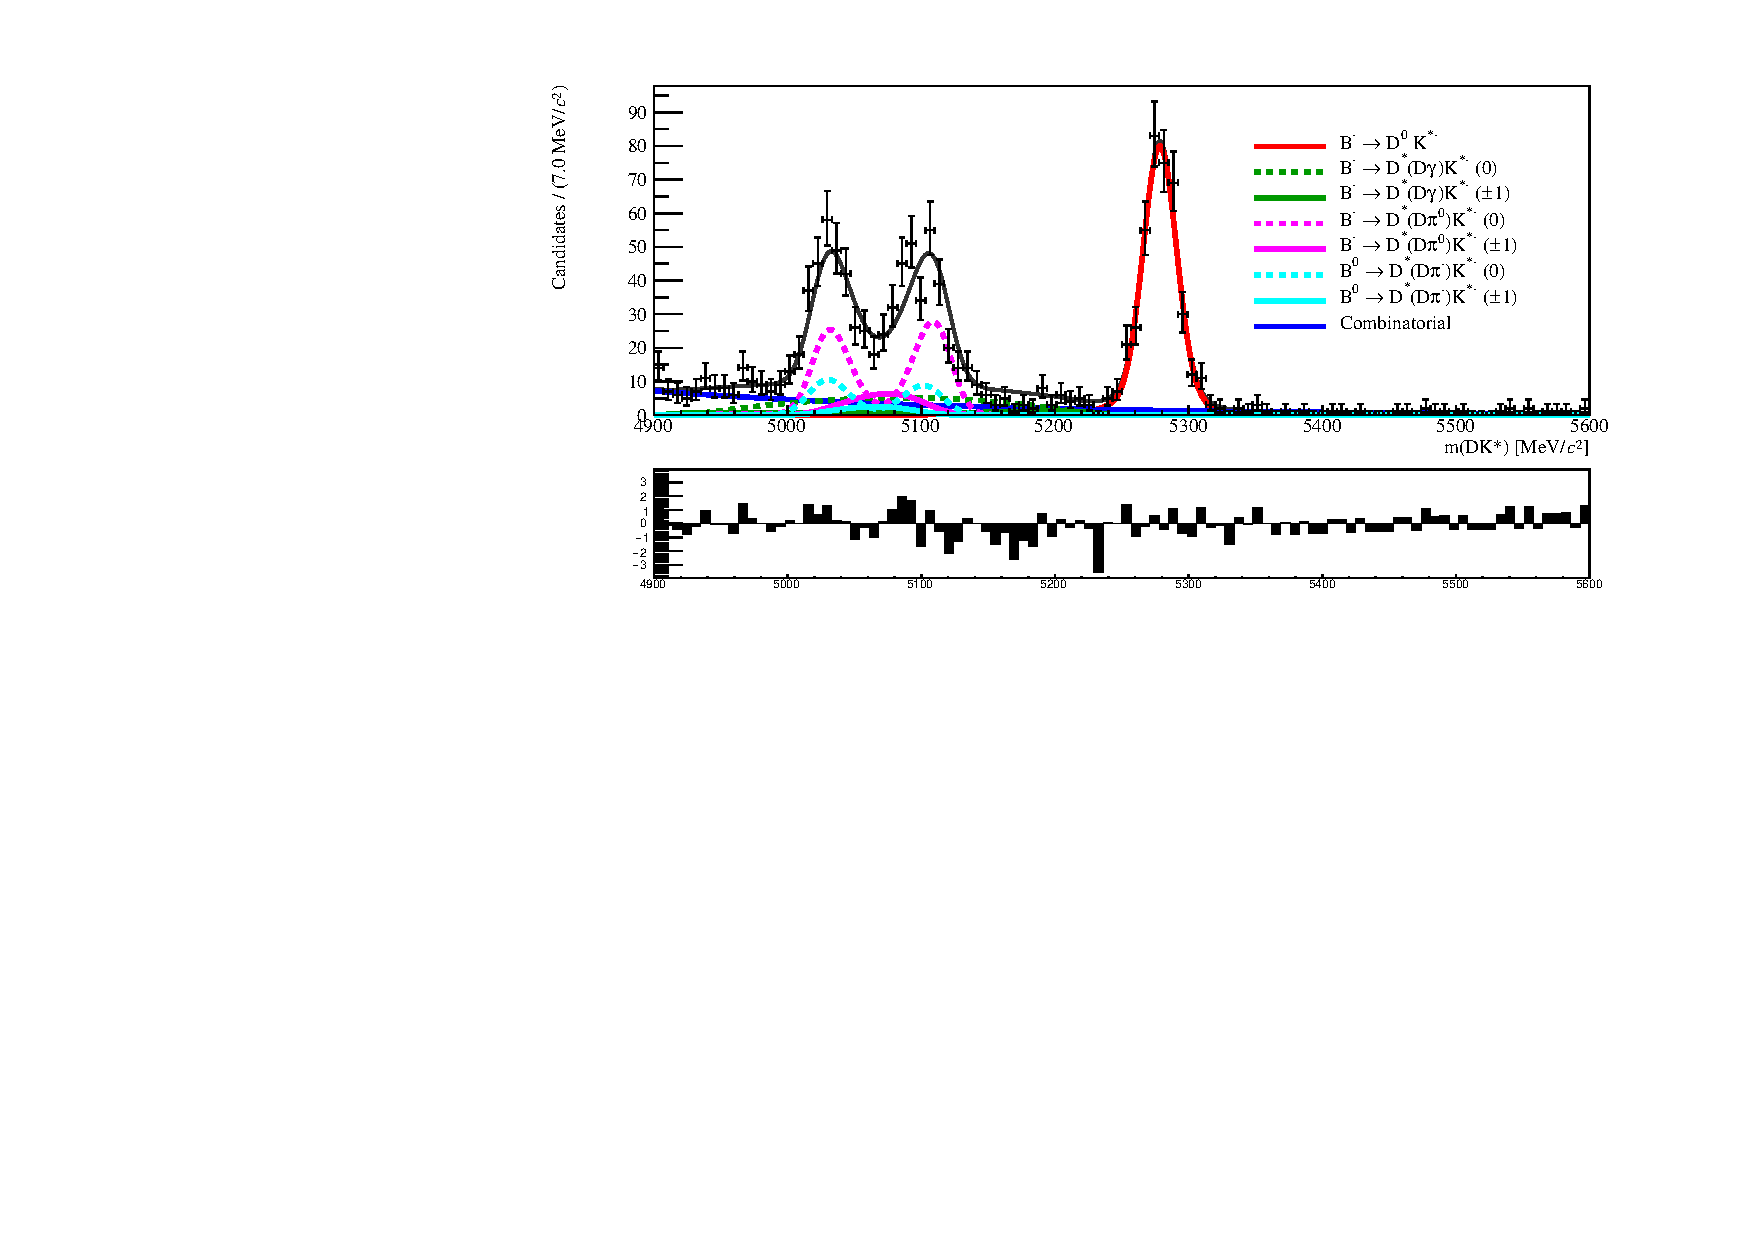
\includegraphics[width=0.7\linewidth]{figures/fitComponents/massFit_LL_KPi_run2.pdf}}
\vspace{-12pt}
\hfill
\subfloat[Run 2 DD]{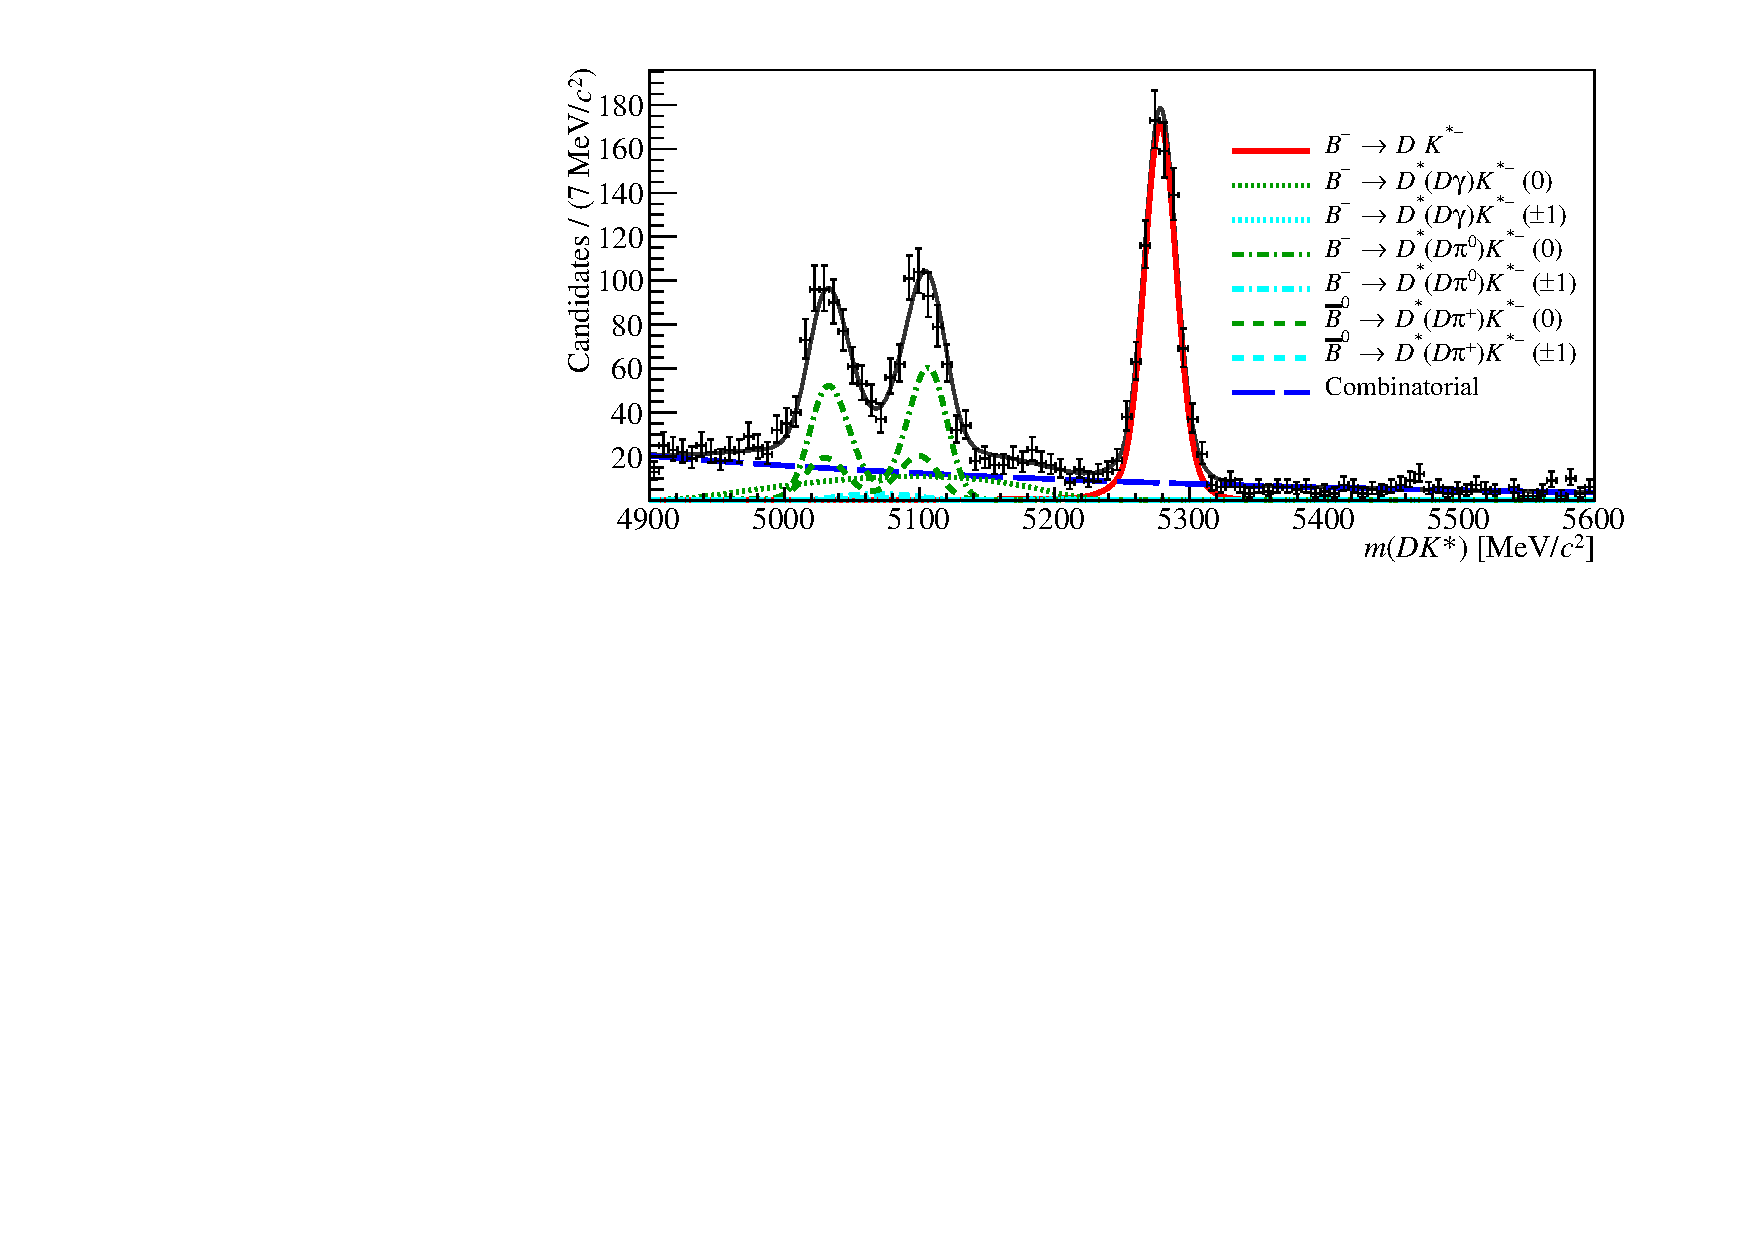
\includegraphics[width=0.7\linewidth]{figures/fitComponents/massFit_DD_KPi_run2.pdf}}
\caption{Fits to the invariant B mass distribution in the $K\pi$ favoured mode}
\label{massfitskpi}
\end{figure}

\begin{figure}
\centering
\subfloat[Run 1 LL]{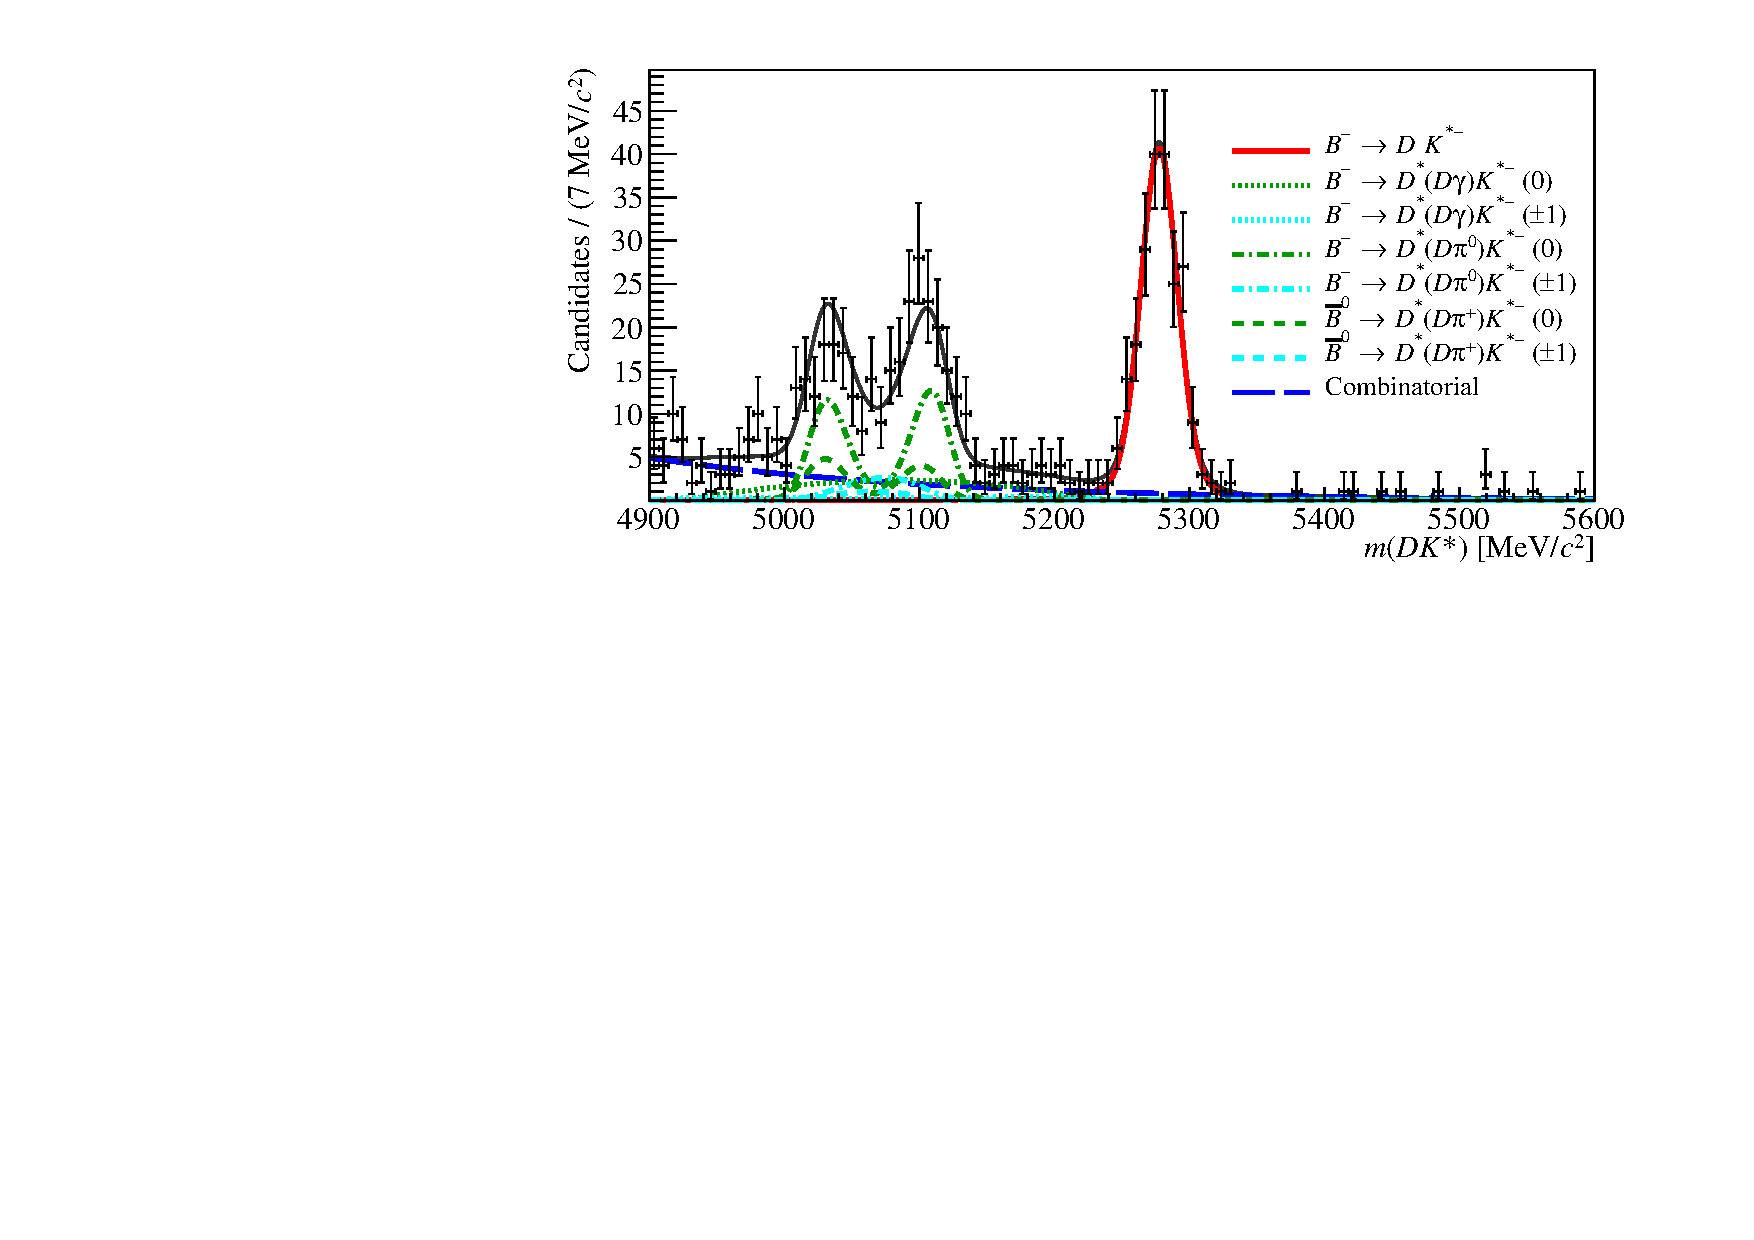
\includegraphics[width=0.7\linewidth]{figures/fitComponents/massFit_LL_KPiPiPi_run1.pdf}}
\vspace{-12pt}
\hfill
\subfloat[Run 1 DD]{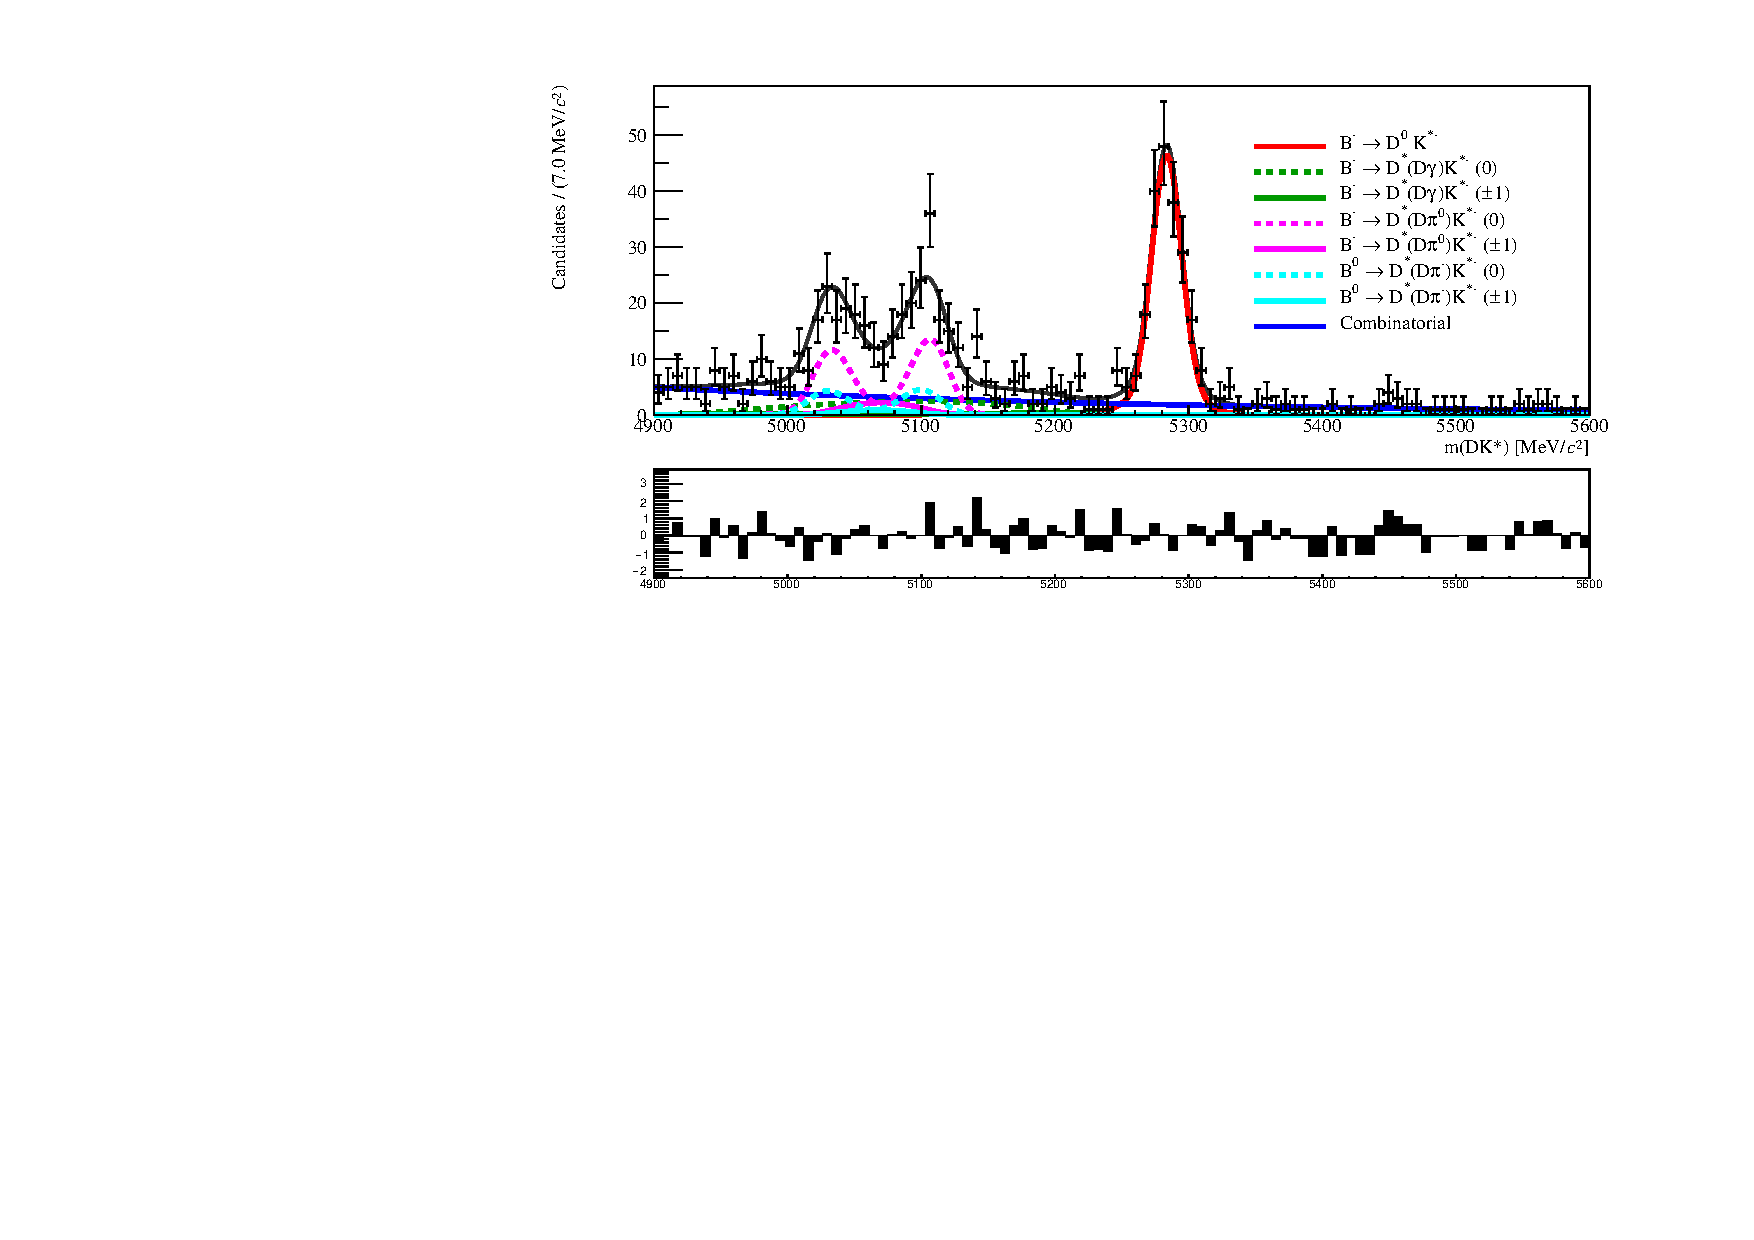
\includegraphics[width=0.7\linewidth]{figures/fitComponents/massFit_DD_KPiPiPi_run1.pdf}}
\vspace{-12pt}
\hfill
\subfloat[Run 2 LL]{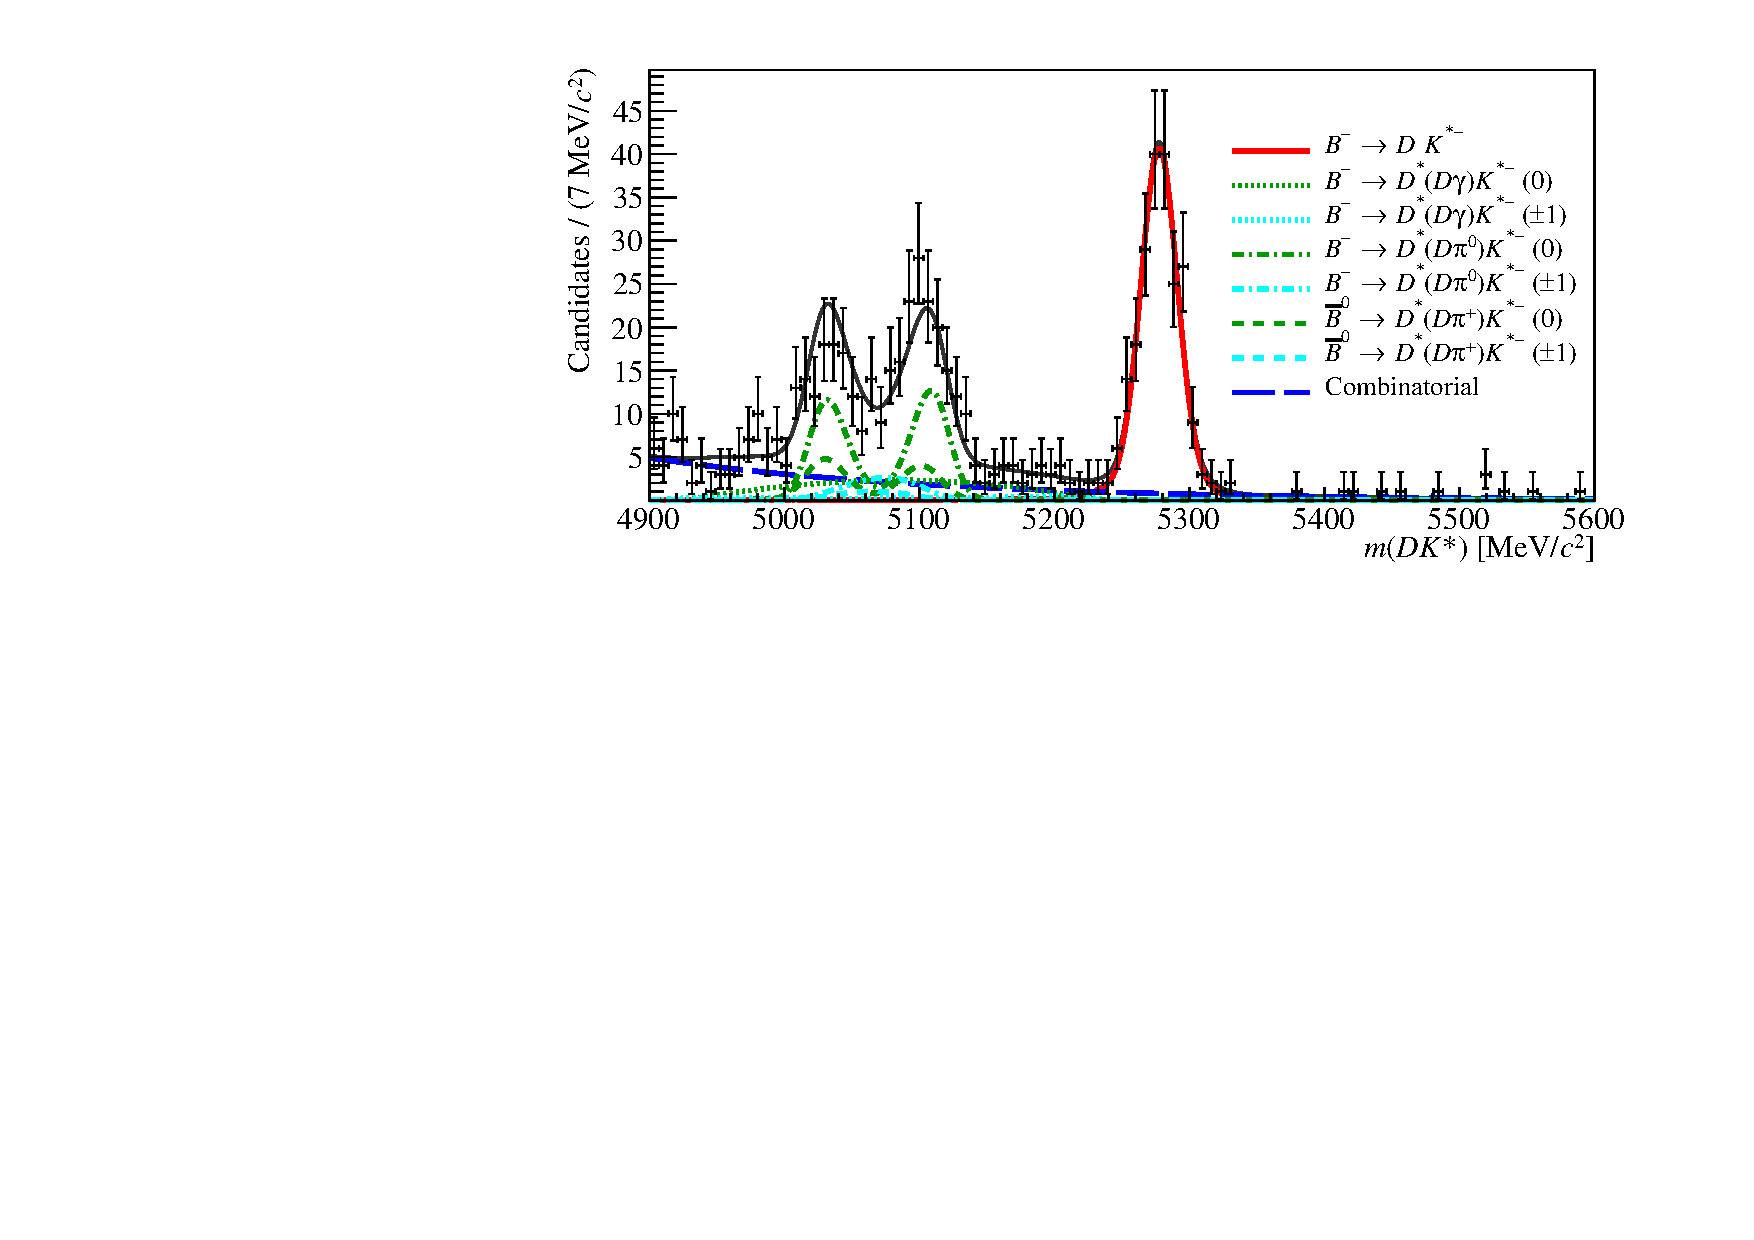
\includegraphics[width=0.7\linewidth]{figures/fitComponents/massFit_LL_KPiPiPi_run2.pdf}}
\vspace{-12pt}
\hfill
\subfloat[Run 2 DD]{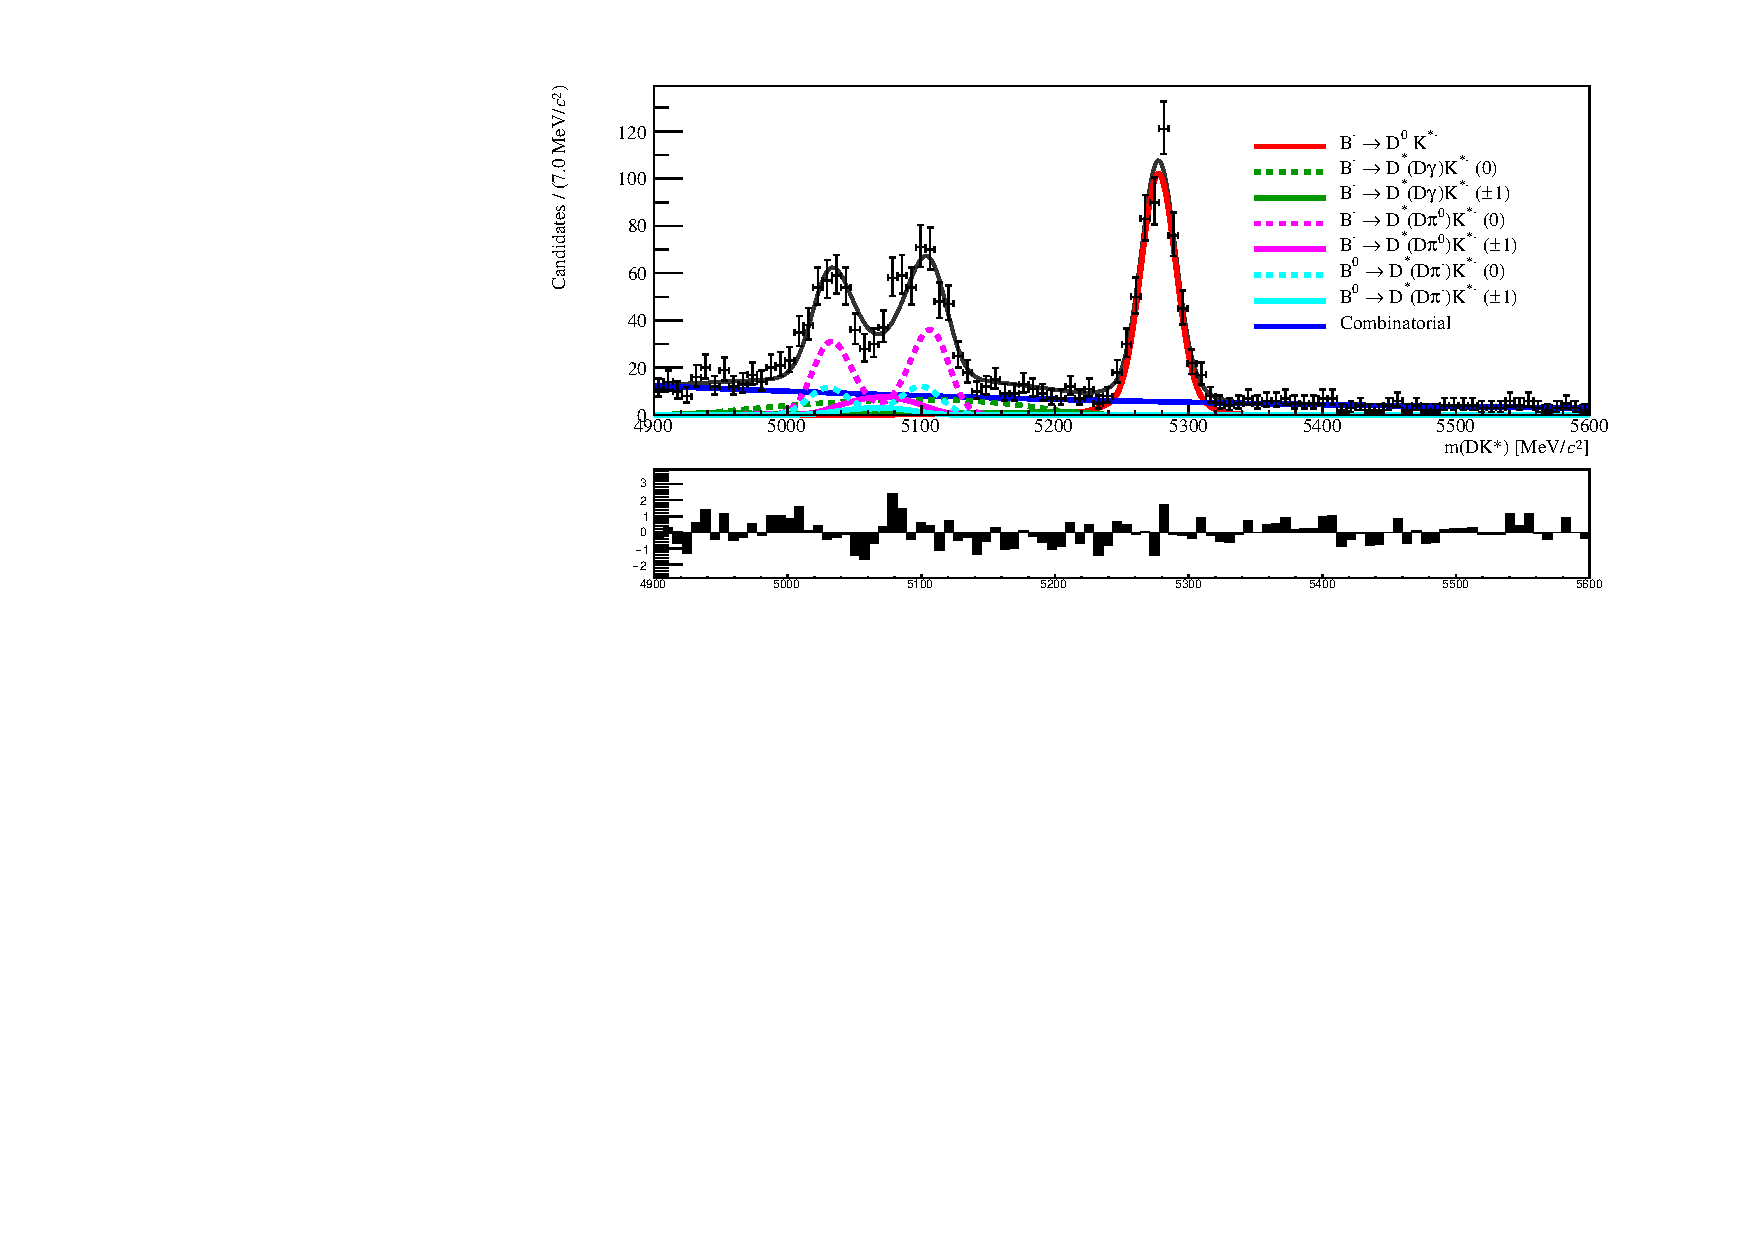
\includegraphics[width=0.7\linewidth]{figures/fitComponents/massFit_DD_KPiPiPi_run2.pdf}}
\caption{Fits to the invariant B mass distribution in the $K\pi$ favoured mode}
\label{massfitsk3pi}
\end{figure}

\begin{table}[h]
\centering
\begin{tabular}{l|cc|cc}
\hline
& \multicolumn{2}{c}{Run 1} & \multicolumn{2}{c}{Run 2} \\
& LL & DD & LL & DD \\
\hline
decay & $(-4.8 \pm 0.5) \times 10^{-3}$ & $(-2.8 \pm 0.3) \times 10^{-3}$ & $(-4.4 \pm 0.5) \times 10^{-3}$ & $(-2.5 \pm 0.2) \times 10^{-3}$ \\
frac\_010 & $0.15 \pm 0.08$ & $0.12 \pm 0.05$ & $0.18 \pm 0.05$ & $0.06 \pm 0.04$ \\
mean & $5280.7 \pm 0.8$ & $5280.7 \pm 0.6$ & $5278.5 \pm 0.8$ & $5278.6 \pm 0.5$ \\
nbkg & $167 \pm 20$ & $472 \pm 34$ & $223 \pm 24$ & $1100 \pm 50$ \\
ndstkst & $338 \pm 23$ & $810 \pm 36$ & $654 \pm 31$ & $1397 \pm 49$ \\
nsig & $220 \pm 16$ & $505 \pm 24$ & $388 \pm 21$ & $901 \pm 33$ \\
sigma & $10.2 \pm 0.7$ & $11.5 \pm 0.5$ & $12.2 \pm 0.6$ & $11.5 \pm 0.4$ \\
\hline
\end{tabular}
\caption{Fit results from the $K\pi$ favoured mode for LL and DD candidates, corresponding to the fits in Figure \ref{massfitskpi}. The parameter $decay$ is the combinatoric background slope, $frac\_010$ is the yield ratio between 010 and 101 helicity amplitudes, $sigma$ is the floating width of the signal shape, and $nsig$, $nbkg$ and $ndstkst$ are the yields of signal, combinatoric background and partially reconstructed decays respectively}
\label{fitresultskpi}
\end{table}

\begin{table}[h]
\centering
\begin{tabular}{l|cc|cc}
\hline
& \multicolumn{2}{c}{Run 1} & \multicolumn{2}{c}{Run 2} \\
& LL & DD & LL & DD \\
\hline
decay & $(-5.2 \pm 1.1) \times 10^{-3}$ & $(-2.3 \pm 0.4) \times 10^{-3}$ & $(-4.4 \pm 0.5) \times 10^{-3}$ & $(-2.1 \pm 0.2) \times 10^{-3}$ \\
frac\_010 & $0.26 \pm 0.11$ & $0.20 \pm 0.08$ & $0.15 \pm 0.07$ & $0.16 \pm 0.05$ \\
mean & $5281.3 \pm 1.3$ & $5283.9 \pm 0.9$ & $5278.7 \pm 1.0$ & $5277.7 \pm 0.7$ \\
nbkg & $50 \pm 12$ & $252 \pm 24$ & $168 \pm 20$ & $707 \pm 40$ \\
ndstkst & $154 \pm 15$ & $317 \pm 24$ & $342 \pm 23$ & $914 \pm 40$ \\
nsig & $102 \pm 10$ & $226 \pm 16$ & $244 \pm 16$ & $578 \pm 27$ \\
sigma & $11.4 \pm 1.0$ & $11.3 \pm 0.8$ & $12.9 \pm 0.8$ & $13.1 \pm 0.6$ \\
\hline
\end{tabular}
\caption{Fit results from the $K\pi\pi\pi$ favoured mode for LL and DD candidates, corresponding to the fits in Figure \ref{massfitsk3pi}. The parameter $decay$ is the combinatoric background slope, $frac\_010$ is the yield ratio between 010 and 101 helicity amplitudes, $sigma$ is the floating width of the signal shape, and $nsig$, $nbkg$ and $ndstkst$ are the yields of signal, combinatoric background and partially reconstructed decays respectively}
\label{fitresultsk3pi}
\end{table}

%%%%%%%%%%%%%%%%%%%%%%%%
\subsection{Choice of fit range}
\label{sec:massfit:range}	

Fixing the relative yields for the partially reconstructed shapes, as in Table \ref{fixedyieldratios}, is possible only under the assumption that \CP violation is negligible. This is a fair assumption for the favoured \decay{\Dz}{\Km\pip} decay, however in the other \D modes, for example \decay{\Dz}{\Kp\Km}, there is expected \CP violation for which the parameters are entirely unknown. Therefore, it is not possible make any constraints at all in these modes. The fit that would result from fitting six individual yields with an order of magnitude less data would be unstable and this lack of constraint in the low mass region would lead to a large amount of freedom in the combinatoric, significantly affecting the signal yield. 

The overlap of the partially reconstructed and signal peaks is very small. There are a number of advantages to raising the lower range of the mass parameterisation up to 5230 \mev, which only removes 0.4\% of signal. The advantages include avoiding the need to fit the various partially reconstructed yields in each of the other D decays modes. These cannot use the same assumptions and fractions as determined in the Cabibbo-favoured mode due to expected CP violation. Further benefits are that low level broad backgrounds that may be present in the range 4900 - 5200 \mev do not need to considered as sources of systematics uncertainty. The shape and yield of the small amount of partially reconstructed background present in all \D decay categories above 5230 \mev is determined and fixed from the fit of data with the Cabibbo-favoured decay, taking into account the smaller branching fractions of the $D$ decays. It is less than an event for all the CP violating modes. Due to the assumptions present in the initial fit, uncertainties in the yield and shape and possible asymmetries in distribution between \Bp and \Bm are evaluated as systematic uncertainties. This systematic uncertainty is dealt with in Section \ref{sec:systematics:partreco}.


\clearpage
